\chapter{鼻和鼻旁窦}

\section{检查方法}

\subsection{常规检查}

鼻和鼻旁窦的CT检查一般可做横断面和冠状面扫描,必要时可行矢状面重建。

横断面扫描:仰卧,去除活动性假牙,以下眶耳线(听眶下线)为基线或以听眦线为基线扫描。从上齿槽开始,向上达额窦水平。层厚、层距为5mm,选择性应用增强扫描,照像应同时有软组织窗和骨窗。

如重点了解薄的鼻旁窦骨壁有否破坏,可用层厚1.5mm、层距5mm扫描,骨算法重建予以观察。

冠状面扫描:垂直于硬腭、听眶下线或听眦线,层厚及层距为5mm。该位置便于观察窦口鼻道复合体,筛窦、蝶窦肿瘤对颅底的影响,以及上颌窦的上下壁。

对以上两种方法的应用各医院不统一,因横断面扫描较为方便,且对显示鼻和鼻旁窦、鼻咽、颅底及颈面深部关系较好,故最常使用。必要时可采取两种扫描方式并用。

\subsection{CT仿真鼻腔镜}

鼻腔和鼻旁窦的CTVE成像应采用轴位扫描,以免受假牙或硬腭等伪影的影响。有学者采用准直3mm,螺距1.0,重建间隔1.0mm,可获得较好的图像。通常采用标准演算法,如欲观察骨质情况则用骨算法。通常,CTVE观察软组织结构的阈值为-600~-200Hu,显示邻近骨质改变则需采用60~100Hu。

CT仿真鼻腔镜能清楚的显示鼻腔、鼻窦和鼻咽部的各种解剖结构和>3mm的占位性病变,可多方位显示息肉或肿瘤的位置、大小、形状、肥大的鼻甲,相应的鼻道狭窄及鼻中隔偏曲,与鼻腔镜基本吻合。并能从后鼻孔观察鼻甲、鼻道狭窄及自后鼻孔突向鼻咽腔的病变。CTVE对鼻咽部的病变也可较好的显示。

\section{正常解剖、变异和CT表现}

\subsection{外鼻}

外鼻呈上窄下宽的三角锥体形,其支架大部分为软骨,小部分为骨。①骨性支架:额骨鼻突、鼻骨和上颌骨额突组成外鼻的骨性支架。②软骨性支架:左右成对的鼻外侧软骨和大翼软骨组成外鼻软骨性支架的主要部分。③梨状孔:由鼻骨下缘、上颌骨内缘和上颌骨额突的游离缘共同围成
。

鼻骨左右成对,中线连接,也可完全缺如而由增大的上颌骨额突代偿。CT不易显示软骨,骨缝呈线形低密度,勿误认为骨折。

\subsection{鼻腔}

鼻腔呈梨形,由鼻中隔分为左右两半,顶窄底宽;前起自梨状孔,后止于鼻后孔通鼻咽部。①鼻前庭:位于前下部。②固有鼻腔:位于后部,前起于鼻前庭的鼻内孔,后止于鼻后孔,为鼻腔的主要部分,可分为呼吸部和嗅部。嗅部包括鼻中隔上部、鼻腔外侧壁上鼻甲以上的部位,约8~10mm范围,其余为呼吸部。每侧鼻腔可有内、外、底、顶4壁。

1.内侧壁:由鼻中隔组成。①软骨部:位于其前部,由鼻中隔软骨及鼻翼软骨内侧脚组成。②骨部:位于后部,由筛骨垂直板和犁骨组成。筛骨垂直板为鼻中隔后上1/3;犁骨位于鼻中隔后下方,其上方与蝶骨及筛骨垂直板相结合,下方与上颌骨鼻棘及硬腭相接。正常人鼻中隔常有弯曲。

2.外侧壁:主要由上颌骨、泪骨、筛骨迷路和蝶骨翼突组成。外侧壁上有3~4个呈阶梯状排列的长条状骨片称为鼻甲,有资料统计3个鼻甲者占16%,而4个者占84%。鼻甲上缘连于外侧壁,下缘呈游离状向内下方呈卷曲状悬垂于鼻腔内,分别称为下、中、上和最上鼻甲。上鼻甲、中鼻甲及最上鼻甲都是筛骨的突起部分。下鼻甲最大,为附着于上颌骨的单独骨块。每个鼻甲的下方有相应的鼻道。上鼻道内有蝶窦和后组筛窦的开口;中鼻道内有前组筛窦、额窦鼻额管和上颌窦开口;下鼻道内有鼻泪管开口;最上鼻道95%有筛后小房的开口。鼻中隔和鼻甲之间的间隙称为总鼻道。冠状面CT可见下鼻甲附着于上颌窦口之下;上鼻甲为附着于筛骨水平板内段的薄骨片;中鼻甲自筛窦顶垂直下降,上端附着于筛板,外侧附着于筛窦内侧壁。横断面上,上鼻甲和上鼻道难与筛窦区分开。

3.顶壁:较窄,宽约5mm,主要由筛骨筛板构成,以薄骨板与前颅窝分隔。

4.底壁:前部为上颌骨腭突,后部由腭骨水平板组成。在鼻底前端骨质较厚和突起称为前鼻棘。在上切牙后方有切牙管,直径一般<5mm,有时上颌窦气化可扩展至腭部,勿误认为囊肿。

5.后鼻孔:上壁为蝶骨体和犁骨翼,内侧为犁骨后缘,外侧为翼突内板,底壁为腭骨。

\subsection{鼻旁窦}

鼻旁窦是与鼻腔相通的含气空腔。按其开口部位可分为两大组:①前组:开口于中鼻道,包括额窦、上颌窦和前组筛窦;②后组:开口于上鼻道,包括后组筛窦和蝶窦(更确切的说蝶窦开口于蝶筛隐窝)。依其位置可分为上下两组:①上组:额窦、筛窦和蝶窦;②下组:上颌窦。上组鼻旁窦病变易累及颅内。

1.额窦:2~3岁开始发育,20岁左右发育完成。其形状、大小个体差异大,可一侧或双侧不发育或过度气化。额窦前壁骨质厚,后壁及底壁(眶上壁)较薄,内壁为中隔,中隔多偏向一侧。

2.筛窦:出生时即有发育,婴儿仅有2~3个气房,发育至20岁时每侧应有3~18个气房。筛骨主要包括两部分:①筛骨骨板:包括水平板、垂直板和纸板;②筛骨迷路:由菲薄的骨板围成的许多小气房组成,可分为前、中、后组小气房。前、中组统称为前组筛窦,后组小气房称为后组筛窦,前后组以基板为界。

筛窦的常见异位气房有:鼻丘气房(上颌骨额突气化)、中鼻甲气房、鸡冠气房、钩突气房、蝶上筛房(Onodi气房)、眶下气房(Haller气房)。

CT横断面和冠状面于每侧有约10个左右气房,并显示上、中鼻甲。横断面可见基板呈弯曲状的自前下向后上斜行,连接于筛窦内外壁之间。

3.上颌窦:出生时即有发育,10岁左右窦底与鼻底在同一水平,15岁以后达成人水平。其呈不规则三角锥体形,尖朝上颌骨颧突,底朝向鼻腔,可分为5个壁。①内侧壁:相当于中鼻道处,大部分为膜性壁,勿误认为上颌窦开口或骨质破坏。上颌窦开口位于内侧壁最高处,骨性窦口由下鼻甲上颌突、泪骨下端、筛骨钩突和腭骨垂直板围成,经筛漏斗流入中鼻道。但窦口可有变异或有副窦口。②前壁:即上颌骨的面壁,眶下缘的下方有眶下孔(有眶下神经和血管通过)。③顶壁:为眼眶的底壁。④底壁:为上颌骨齿槽突,是上颌窦最后气化发育的部分。⑤后外侧壁:与颞下窝和翼腭窝毗邻。有时可见外侧壁上的后上齿槽神经血管沟呈裂隙状,勿误认为骨折。

4.蝶窦:2~3岁发育,青春期后发育完全。大小、形态个体差异大,气化好者可伸向蝶骨大翼、翼突根部、筛窦区扩展。左右常不对称,骨性间隔偏向一侧。可分为顶壁、底壁、前壁、后壁、内侧壁和外侧壁。前壁之骨性窦口直径约10mm,覆盖黏膜的窦口直径约2~3mm。

\subsection{窦口鼻道复合体}

窦口鼻道复合体通常包括中鼻甲、筛泡、筛漏斗、半月裂、钩突及中鼻道,前组鼻窦均开口于此。该区是呼吸气流的主通道,是炎症和息肉的始发和多发区。除病变外,该区的解剖变异也可导致开口狭窄或闭塞,使之引流不畅,反复感染,最后演变为前组鼻旁窦慢性炎症。

国外学者将上述窦口鼻道复合体称为前窦口鼻道复合体,而将蝶筛隐窝和上鼻道称为后窦口鼻道复合体。但大多数学者所指窦口鼻道复合体即前者(图\ref{fig5-1})。

\begin{figure}[!htbp]
 \centering
 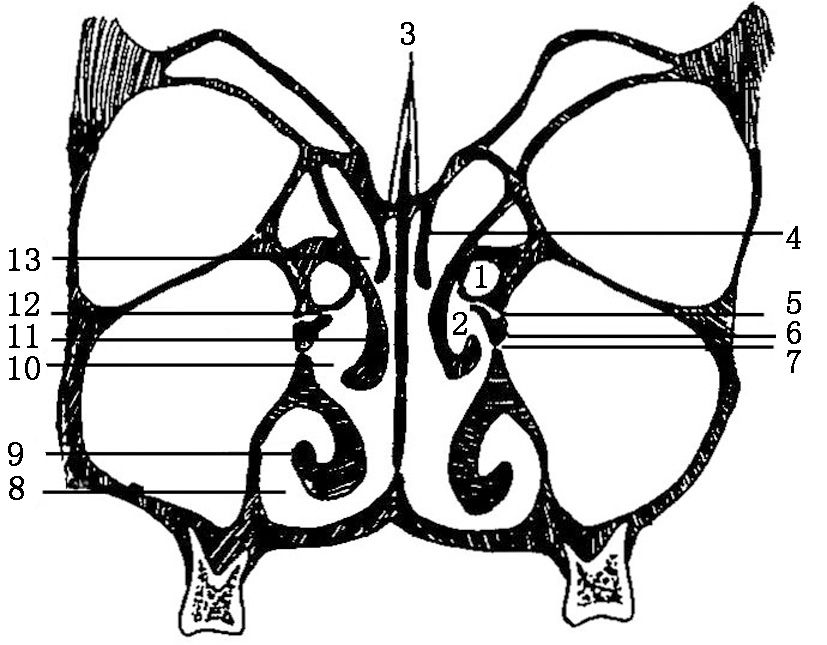
\includegraphics[width=.7\textwidth,height=\textheight,keepaspectratio]{./images/Image00122.jpg}
 \captionsetup{justification=centering}
 \caption{鼻腔和鼻旁窦冠状位\\{\small 1.筛泡;2.半月裂;3.鸡冠及筛板;4.上鼻甲;5.上颌窦口;6.钩突;7.上颌窦副窦口;8.下鼻道;9.下鼻甲;10.中鼻道;11.中鼻甲;12.筛漏斗;13.上鼻道}}
 \label{fig5-1}
  \end{figure} 

窦口鼻道复合体区重要的解剖标志如下:

1.鼻丘气房:位于中鼻甲前上附着处的前方,额隐窝的前面,为上颌骨额突的骨性突起气化而成,是鼻腔外侧壁最前面的异位筛窦小房,可伸展至泪骨。鼻丘气房引流入筛漏斗,可阻塞额隐窝。

2.钩突:是来自筛骨迷路、附着于下鼻甲筛突上的、镰刀状薄骨板,形成鼻腔外侧壁的一部分。前与泪骨相连,弯曲向下后经过上颌窦窦口上缘游离,下端同下鼻甲的筛突相连,游离缘形成半月裂的内侧缘,钩突向后下发展形成半月裂的下缘和筛漏斗的内侧缘,其大小变异很大。

3.筛漏斗:为一槽形腔道,位于筛泡之下、钩突上外方,最前方在鼻丘气房下面和钩突前部的上方。钩突亦可连接筛骨纸板,在这种情况下筛漏斗上端呈一盲囊,称为终末隐窝。

4.半月裂:来自筛漏斗的弯沟,位于钩突之上、筛泡之下,经越上颌窦自然开口,在下鼻甲后上方逐渐消失,为筛漏斗通向中鼻道的裂口。

5.筛泡:为中组筛窦中的一个大气房,位于中鼻道外侧壁。

6.额隐窝:额窦经鼻额管进入中鼻道,此管是额窦和中鼻道前端间一内在管道。位于前组筛小房的裂隙称为额隐窝或筛漏斗的额隐窝,额窦开口于额隐窝的最前上方。

\subsection{鼻及鼻窦的解剖变异}

1.上颌窦的变异:①上颌窦发育不全:包括体积变小、上颌窦底壁高于鼻底。较重的发育不全,窦腔较小、骨质增生硬化较厚、黏膜肥厚,并有钩突发育不全。②上颌窦分隔:可分为纤维或骨性分隔,分隔常从眶下管到窦的外侧壁。

2.鼻甲气化和鼻中隔弯曲:鼻甲气化又称为泡状鼻甲,以中鼻甲气化为多;鼻中隔弯曲可呈“〉”、“C”或“S”型弯曲。上述变异可压迫和阻塞鼻道引发鼻窦炎。

3.蝶窦的变异:①气化可扩展到前床突、翼突,分别称为前床突气化和翼突气化。过度气化可增加视神经、圆孔等暴露的机会,蝶窦手术时应予注意。②蝶窦分隔正常应为二分隔,可为纤维性和骨性,亦可无分隔。三分隔变异术前应提示,否则易导致手术后病变残留。③蝶窦发育不良多呈甲壳状,窦腔变小。

4.蝶上气房(Onodi气房):是指后组筛房向后延伸包绕视神经管和视神经;向蝶窦外上方延伸,与蝶窦共壁;并向上达蝶鞍的前壁,前床突与蝶窦间以筛板相隔。该气房增加鼻内镜手术对视神经损伤的机会。

5.眶下气房(Haller气房):是位于筛泡下方沿上颌窦顶壁和筛骨纸板最下部分的任何气房,包括筛漏斗的气房。可使筛漏斗及上颌窦口变窄,引发上颌窦及额窦炎症。

6.筛泡过大、钩突气化、钩突偏斜和钩突肥大、中鼻甲反向、鼻中隔气化等变异均是引发鼻窦炎及鼻窦炎经久不愈的原因。

\subsection{颞下窝}

又称咀嚼肌间隙,位于颅底下,以颧弓和蝶骨大翼上的颞下嵴为界,以上为颞窝,以下为颞下窝。颞下窝的界限:①上界为颅底即蝶骨大翼和岩骨尖;②前界为上颌窦后壁,翼腭窝和翼内、外板;③后界为颈鞘和茎突;④外界为下颌支、下颌小头、冠状突和颞肌;⑤内界为鼻腔和鼻咽部。此窝上通颞窝,借卵圆孔和棘孔与颅中窝相通,向后通翼腭窝。横断面CT示颞下窝内充满低密度脂肪块,后外侧为呈条束状中等密度影的颞肌。翼突内、外板外侧附有中等密度的翼内肌和翼外肌。

\subsection{翼腭窝}

翼腭窝是颞下窝向前、内的延伸,即蝶骨体、蝶骨翼突、上颌窦后壁、腭骨垂直板及颞下窝围成的小间隙。前界为上颌窦后壁,后界是翼突,内界为腭骨。翼腭窝内有蝶腭神经节、三叉神经上颌支和上颌动脉的终末支及其伴随静脉。前部包括所有的血管成分,后部为神经所在部位。这些结构由疏松结缔组织和大量脂肪包绕,因此CT可以显示。横断面CT示其内为低密度脂肪,增强可见上颌动脉分支,神经常不能显示。冠状面有时可见神经呈圆形软组织结构。

此窝的通连关系:①向后上经圆孔通颅中窝;②向前上经眶下裂通眼眶;③向内侧经蝶腭孔通鼻腔;④向下经腭大管及腭小管通口腔;⑤向后下经腭鞘管通鼻咽部;⑥向后经翼管通破裂孔;⑦向外侧经翼上颌裂通颞下窝。

腭鞘管由腭骨的蝶突和蝶骨鞘突形成,位于翼管内下方、鼻咽的顶部。管内有腭鞘动脉(为上颌内动脉向后的一个分支)及咽神经(从蝶腭神经节到咽鼓管咽口)。腭鞘管横断面和冠状面HRCT均可显示,横断面呈窄锥形;冠状面多呈圆形或卵圆形(其下壁骨质可不完整)。

\section{先天性疾病}

\subsection{先天性后鼻孔闭锁}

本病为鼻后孔的先天性发育畸形,可单侧或双侧发生,但多为单侧,可完全性或部分性,病因尚不完全明确。

\textbf{【病理】}
可为膜性、软骨性、骨性或混合性,以骨性和混合性多见,占80%~90%,其次为膜性,软骨性极少。闭锁隔一般由鼻腔黏(骨)膜、鼻咽黏(骨)膜和中间的骨板组成,大多周边厚而中央有一小凹陷,有时中央留小孔。其厚薄不一,为1~12mm,多在2mm左右。常伴多指趾、颅面畸形、眼和消化道畸形等。

\textbf{【临床表现】}
双侧闭锁者出生后即有呼吸困难,啼哭时症状减轻,常因窒息而死亡。单侧者表现为鼻塞、鼻内分泌物增多、打鼾等。年龄大者表现为鼻塞、张口呼吸、鼻音等。

\textbf{【CT表现】}
可清楚的显示闭锁的部位、厚度,闭锁隔为骨性或膜性。骨性者见鼻中隔后端及鼻后孔外侧骨质增厚,鼻后孔狭小或闭锁。有时骨质增生可涉及到腭骨、蝶骨体或翼突内侧板。

\textbf{【鉴别诊断】}
①后天性粘连瘢痕狭窄:多有特殊感染(如结核、梅毒等)、外伤、手术、放疗等病史。②先天性鼻腔狭窄:较先天性后鼻孔闭锁少见,CT可见鼻腔中部骨性增生导致鼻腔狭小。③后鼻孔息肉:呈类圆形或结节状软组织肿块。④增殖体肥厚:多为鼻咽顶后壁弥漫性较高密度软组织增生,表面不平。

\subsection{先天性鼻背囊肿和瘘管}

本病占头颈部(上)皮样囊肿的8%~12.8%。

\textbf{【病理】}
其发病机制多种多样,但认为是胚胎早期外胚层被包埋的结果。病灶无窦口与外界相通者为囊肿;与外界直接有窦口相通者称为漏管;漏管一端膨大呈盲端者称为窦。囊肿内含上皮及脱屑者为上皮样囊肿;而含有真皮的汗腺、皮脂腺、毛囊等皮肤附件者为皮样囊肿。

\textbf{【临床表现】}
多为婴幼儿,男性多见,家族遗传少见。囊肿浅在者鼻梁膨隆,深在者使鼻中隔膨大。形成瘘管者可在鼻背部皮肤有针孔状开口及分泌物排出。多有鼻背脓肿反复发作史。

\textbf{【CT表现】}
病灶几乎都位于鼻中线,可发生于鼻额缝至鼻小柱基底间的任何部位,最常见于鼻中隔骨与软骨交界处。囊肿表现为鼻背软组织肿大膨隆,皮下可见低密度软组织影,有明显包膜,边缘光滑。若有感染囊液密度增高,包膜界限不清,并可增厚。鼻骨和鼻中隔可有骨吸收或分叉变形,若病变向上扩展可致鸡冠分叉变形或偏位。此外,瘘管、窦道的显示以X线造影为佳。

\subsection{鼻胶质瘤}

本病属先天性少见疾病。

\textbf{【病因病理】}
其发生原因与脑膜膨出相似,不同之处为颅底脑膜及骨缺损处在胚胎期已基本自然愈合,使得一部分脑组织遗留于鼻部,与颅内多无直接连接或仅以纤维带连接,故认为是先天性发育异常,而非真正肿瘤。鼻胶质瘤可分为3型:①鼻外型:占60%,肿块位于鼻根或鼻旁;②鼻内型:占30%,肿块位于鼻腔顶部;③混合型:占10%,以上两者均有。

\textbf{【临床表现】}
鼻外型多在婴幼儿的外鼻或鼻旁出现质硬肿块。鼻内型多位于鼻腔顶部,可至成人时被发现或误为息肉,也可伴脑脊液鼻漏。

\textbf{【CT表现】}
肿块呈实质性与脑组织密度相仿,位于外鼻或鼻腔顶,偶见鼻外与鼻内肿块相连。鼻内肿块基蒂可通过盲孔与前颅窝相连或经缺损的筛板延伸于前颅窝底。附近鼻骨或额骨多有缺损,鼻中隔可移位。鸡冠可偏位,眶间距亦可增宽。

\textbf{【鉴别诊断】}
①脑膜脑膨出:临床表现多柔软透亮、有弹性,啼哭用力、压迫颈静脉肿块可增大,穿刺有脑脊液。影像学表现为骨缺损较大,位于鸡冠前后,鞘内注射造影剂后肿块显影。②应注意与血肿、脓肿、囊肿、血管瘤、鼻息肉等相鉴别。

\subsection{鼻部脑膜膨出或脑膜脑膨出}

本病是指脑膜或(和)部分脑组织经过鼻额部或颅底未发育完全或钙化不全的骨缺损处疝至颅外而构成的先天畸形。

\textbf{【病理】}
脑膜膨出内容物含有脑膜和脑脊液;脑膜脑膨出内容物含脑组织和脑膜;最重者脑室前角也可膨出称为脑室脑膨出,一般分为前顶组和颅底组。

\textbf{【临床表现】}
多见于婴幼儿,在鼻外部骨缺损处可见圆形或椭圆形肿块。患儿啼哭或压迫颈内静脉时该肿块可增大或张力增加。肿块触之柔软,表面光滑,有的可见搏动等表现。

\textbf{【CT表现】}
可明确显示骨缺损的部位、疝口的大小和形态,软组织肿块的大小、范围及与颅内交通情况。鼻部脑膜膨出或脑膜脑膨出表现为,平扫在鸡冠前可见中等密度软组织肿块,常向下突入鼻腔或筛小房内。鸡冠前的盲孔有时可见扩大,鸡冠可有骨质吸收或分叉。骨缺损部位多呈类圆形,边缘光滑、膨胀、硬化。增强扫描脑膜脑膨出者,脑组织与正常脑组织的强化一致。

\section{外伤}

\subsection{鼻骨骨折}

鼻骨骨折是面部最常见的骨折,可仅为单纯骨折,亦可为多发粉碎性骨折,还可伴有其他面部骨折。鼻骨骨折常发生于鼻骨中下段。鼻骨多发粉碎性骨折,可涉及到上颌骨额突、泪骨、鼻中隔,并可伴有泪骨移位,筛房及纸板、额骨眶突骨折。

\textbf{【CT表现】}
鼻骨骨折一般采用X线平片诊断即可。CT检查应螺旋扫描并以1~2mm层厚重建才可能显示单纯性骨折,否则难以显示轻微的单纯骨折,亦难以区分是否为粉碎性骨折(图\ref{fig5-2})。横断面与冠状面综合观察,更有利于显示骨质中断的骨折线及断端移位方向、程度等。我们通常对法医鉴定者进行三维重建,以进一步提高诊断准确性。

\begin{figure}[!htbp]
 \centering
 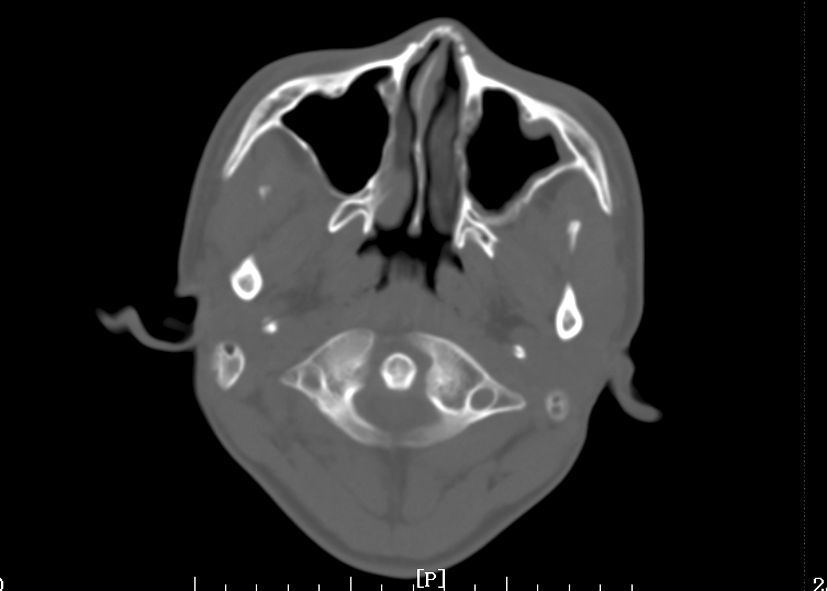
\includegraphics[width=.7\textwidth,height=\textheight,keepaspectratio]{./images/Image00123.jpg}
 \captionsetup{justification=centering}
 \caption{鼻骨骨折\\{\small 鼻骨有多条骨折线,右侧鼻上颌骨额突缝略分离}}
 \label{fig5-2}
  \end{figure} 

总之,正确区分骨折的位置、程度(是否粉碎或复合骨折等)、移位方向及邻近颅缝有否分离等涉及法医学鉴定,应予重视。

\textbf{【鉴别诊断】}
上颌骨额突骨折以横断面显示最佳。通过观察鼻上颌骨额突缝的位置,不难区分骨折位于鼻骨或上颌骨额突,进而观察鼻上颌骨额突缝是否有分离(图\ref{fig5-3})。

\begin{figure}[!htbp]
 \centering
 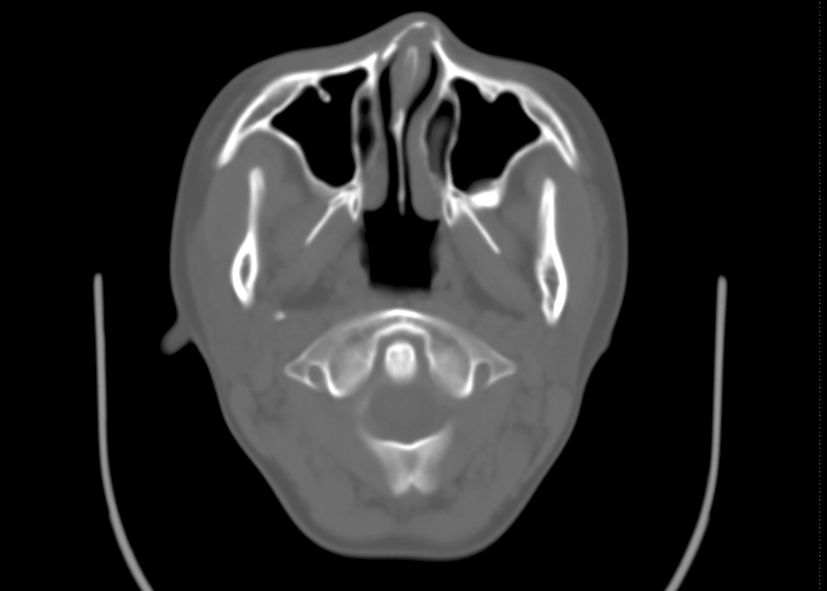
\includegraphics[width=.7\textwidth,height=\textheight,keepaspectratio]{./images/Image00124.jpg}
 \captionsetup{justification=centering}
 \caption{右侧上颌骨额突骨折\\{\small 右侧上颌骨额突有骨折线,左侧鼻上颌额突缝分离}}
 \label{fig5-3}
  \end{figure} 

\subsection{三角架骨折}

三角架骨折或称三联骨折或颧骨上颌骨骨折,包括3处骨折:①眼眶外壁骨折:骨折线通过额颧缝;②眶底骨折:骨折线通过眼眶前下缘,进入上颌窦,累及上颌窦外侧壁;③颧骨弓骨折。

此外,可有上颌窦窦腔积血或黏膜肿胀及眼外、下直肌肿胀。

\subsection{Lefort骨折}

Lefort骨折是涉及双侧上颌骨的面中部骨折,可分为3型。

Ⅰ型:为中面部下区或上颌横行骨折。骨折线于牙列上方、向两侧延伸,经过齿槽骨、梨状孔侧缘、上颌窦下部、腭骨,后延至翼突下部。

Ⅱ型:为上颌骨锥形骨折。骨折线在两侧经鼻骨下部、上部额突、筛骨、泪骨,斜向下延伸至眶下缘------眶底(颧颌缝)和上颌骨,终止于翼突,一般不涉及颧骨。

Ⅲ型:为颅面骨分离骨折。骨折位置高,经额骨下部、筛骨、蝶骨和眼眶,后延伸至翼突上部,常致鼻额缝、颧额缝分离并涉及颅底。

有时这类骨折可双侧不对称,或Ⅱ、Ⅲ型结合存在,多见于额筛区粉碎性骨折者。

\subsection{筛窦骨折}

筛骨纸板菲薄,外伤时易发生骨折。

筛窦骨折可分为3类:线状、凹陷和粉碎性。以眶内壁的筛骨纸板骨折最常见,平片不易显示。眶内壁凹陷性骨折多见于爆裂骨折,常与眶底骨折伴存。粉碎性骨折和Lefort骨折多涉及邻近结构。

\textbf{【CT表现】}
可清楚显示骨折线和骨片移位,筛窦气房密度增高,有的可伴眶内积气,眶内侧软组织肿胀,内直肌移位或粘连。凹陷骨折者常有眶内脂肪和眼外肌嵌顿、外疝。如骨折累及筛窦顶壁板,还可出现颅内积气或脑脊液鼻漏。

\subsection{额窦骨折}

额骨骨折多涉及额窦前壁,少数延及后壁或伴有前颅窝底骨折,可分为线型、凹陷型和粉碎型骨折。

\textbf{【CT表现】}
无论线状或凹陷性骨折,均常见额窦密度增高或积液。额窦后壁骨折可伴颅内积气,甚至硬膜外出血或额叶脑挫裂伤。额窦下壁骨折多损及鼻额管,继而可导致黏液囊肿发生。有的骨折可延伸至筛板和眶顶额骨水平板,亦可发生脑脊液鼻漏和眶内软组织损伤。

\subsection{蝶窦骨折}

蝶窦骨折多为额、筛窦区或颅底骨折延伸引起,故常为复合骨折。

\textbf{【CT表现】}
可见骨折线涉及窦壁,窦内有血液平或黏膜肿胀。还可显示蝶窦邻近的骨折,可导致视神经和眼运动神经损伤、脑脊液鼻漏。海绵窦动静脉瘘或假性动脉瘤形成需增强或造影进一步确诊。

\subsection{外伤性脑脊液鼻漏}

鼻腔与之相关的鼻旁窦和咽鼓管等处与脑脊液之间均有骨板和硬脑膜相隔,当外伤骨折时可使此处的硬脑膜破裂而致脑脊液直接或间接流入鼻腔或鼻旁窦导致脑脊液鼻漏。前颅窝骨折多涉及额、筛窦,中颅窝骨折还可涉及蝶窦顶壁。外伤性多在伤后立即发生,也可在外伤一段时间后发生,后者称为迟发性脑脊液鼻漏,迟发性原因不清。

\textbf{【CT表现】}
平扫不能直接发现脑脊液鼻漏的具体位置,却可清楚的显示颅底骨折的部位、骨折片移位情况。骨折邻近的鼻旁窦密度可增高,内有积液和液平,可间接提示脑脊液鼻漏的位置。腰穿行脑池造影可见造影剂从骨折处流入鼻腔或鼻旁窦内,从而明确瘘口的位置和大小。

\section{炎症和囊肿}

\subsection{概述}

鼻腔和鼻旁窦的关系密切,且两者黏膜相延续,故鼻炎伴发鼻旁窦炎临床上很常见。鼻炎不需影像学检查,鼻窦炎需影像学检查诊断。临床上无明显症状而影像学检查可发现鼻旁窦有异常改变者X线平片约20%,CT约40%,而MR则高达60%。

\textbf{【分类】}
鼻和鼻旁窦炎症依其病因可分为:①化脓性炎症;②过敏性炎症;③特源性炎症(结核、真菌、梅毒、麻风、红斑狼疮、鼻硬结病等)。依其病程有:①急性炎症;②慢性炎症。炎症可发生于一个、一侧或双侧多个窦腔或全部窦腔,且程度可有不同。

\textbf{【CT表现】}
①窦腔内密度增高,黏膜增厚,有软组织影,亦可有气液平面;②窦壁骨质增生硬化、增厚或骨质稀疏,亦可有骨质破坏;③CT可显示鼻源性眶内并发症和颅内并发症、骨髓炎以及其他周围炎性病变。

\subsection{鼻腔和鼻旁窦结石}

鼻结石大多发生于鼻腔内,少数可见于鼻咽或上颌窦内。

\textbf{【病因病理】}
有外源性和内源性之分。分别以外源性异物(如纽扣、纸片、棉花等)或内源性异物(如鼻内分泌物干结凝块或异位牙齿等)为核心,异物存留时间较久后,周围炎性渗出物中的钙、磷等物质沉积,逐渐形成结石。其大小不等,有时可双侧发生或多发。

\textbf{【CT表现】}
鼻腔或鼻旁窦内有类圆形致密钙化灶,其核心密度可高可低。鼻窦结石多发生于上颌窦内,多由鼻腔结石过多而侵及形成。

\subsection{气压性鼻旁窦炎}

本病又称鼻旁窦气压性损伤,为大气压急骤变化时发生鼻窦渗出性反应及出血,见于航空、潜水或沉箱工作人员。

\textbf{【病因病理】}
当人体处于大气压急骤变化的环境下,如鼻旁窦开口通畅,保持窦内外压力平衡,不会发生病变;如鼻旁窦解剖异常(如鼻中隔偏曲)或有病变(如黏膜增厚或息肉),可使窦腔内压力低于体外压力,以致黏膜血管扩张、渗出,间质内体液积聚,黏膜弥漫性水肿,甚至可发生黏膜剥离、黏膜下血肿形成。

\textbf{【临床表现】}
一般多在飞机下降或潜水下沉,大气压升高时发生。主要表现为突发性额部或面颊部疼痛,飞行者以额窦发生为多,潜水者以上颌窦为多。其损伤程度与压力差大小及发生速度有关。一般症状在数周内消失,如继发感染可转为化脓性炎症。

\textbf{【CT表现】}
主要改变为额窦和上颌窦内黏膜肿胀增厚,甚至可见整个窦腔密度增高。有时可见到液平面。重者见黏膜下血肿,形似黏膜下囊肿,可单发或多发,大小不等,大者可充满窦腔。窦腔形态及窦周骨质一般无异常改变。

\subsection{化脓性鼻旁窦炎}

本病为常见多发病,通常按病理分为急性和慢性。慢性者远较急性多见,主要因急性者反复发作或持续性炎症迁延不愈而转变成慢性,但牙源性上颌窦炎可慢性起病。

\textbf{【病因】}
感染多来自鼻腔,少数可来自咽部(如增殖体和扁桃体炎症)和牙。上呼吸道感染、变态反应性炎症、外伤、异物、游泳或潜水时污水灌入鼻窦、理化因素的刺激等为其诱因。局部因素如窦口鼻道复合体解剖变异、肿块阻塞等妨碍引流也是其诱因。此外,全身因素如营养不良、机体抵抗力差等对炎症的发生和发展也有影响。

\textbf{【病理】}
①急性:表现为黏膜充血、肿胀和脓性分泌物产生。如机体抵抗力差,感染可向窦周发展,导致眶面甚至颅内并发症。②慢性:黏膜慢性炎性充血肿胀、腺体增生和血管新生可致黏膜增厚、黏膜腺阻塞可形成潴留囊肿,并可形成息肉样变增厚或息肉。窦壁骨膜、骨质常有反应性增生。

\textbf{【临床表现】}
主要为鼻塞、流脓涕、头痛及局部压痛。上颌窦及蝶窦炎头痛可表现为上午轻、下午重,额窦及筛窦炎头痛则可表现为上午重、下午轻。急性者多有全身不适、发热;慢性者多无全身症状。

\textbf{【CT表现】} 急、慢性化脓性鼻旁窦炎表现如下:

1.急性:发病后1~2天内可无任何阳性征象。随病情进展鼻腔和鼻旁窦黏膜肿胀增厚,一般与窦壁平行;窦腔内分泌物常出现液气平面。窦壁骨质一般无异常,少数可致骨皮质吸收。增强后常见增厚的黏膜下层呈线状强化,而窦内积液不强化。

并发症:如炎症未被控制可出现眶和面部蜂窝组织炎、骨膜下脓肿、骨髓炎等眶面部并发症。还可导致脑膜炎、静脉窦血栓性炎症、脑炎或脑脓肿等颅内并发症。

2.慢性:窦壁骨质硬化增厚是慢性特点,也是与急性或过敏性鼻旁窦炎的鉴别要点。黏膜增厚,可伴黏膜囊肿或息肉形成,但囊肿小、可多发,与小息肉常难以鉴别(图\ref{fig5-4})。窦腔内可见液气平面,急性发作时积液增多。窦腔内如被息肉充满,可致窦腔扩大,甚至骨质破坏。增强扫描黏膜下层可呈线状强化,息肉亦可强化,而积脓不被强化。

\begin{figure}[!htbp]
 \centering
 
\includegraphics[width=.7\textwidth,height=\textheight,keepaspectratio]{./images/Image00125.jpg}
 \captionsetup{justification=centering}
 \caption{慢性化脓性上颌窦炎\\{\small 左右侧上颌窦黏膜呈环状显著增厚;左右侧下鼻甲肥大,以右侧显著}}
 \label{fig5-4}
  \end{figure} 

并发症:可导致眶内炎性假瘤、颌面骨慢性骨髓炎等。

此外,应注意冠状面扫描观察有否窦口鼻道复合体的解剖变异,有利于鼻腔镜手术方案的制定。

\textbf{【鉴别诊断】}
化脓性鼻旁窦炎主要应与过敏性鼻旁窦炎相鉴别(见表\ref{tab5-1})。

\begin{table}[htbp]
\centering
\caption{过敏性鼻旁窦炎与化脓性鼻旁窦炎的鉴别诊断}
\label{tab5-1}
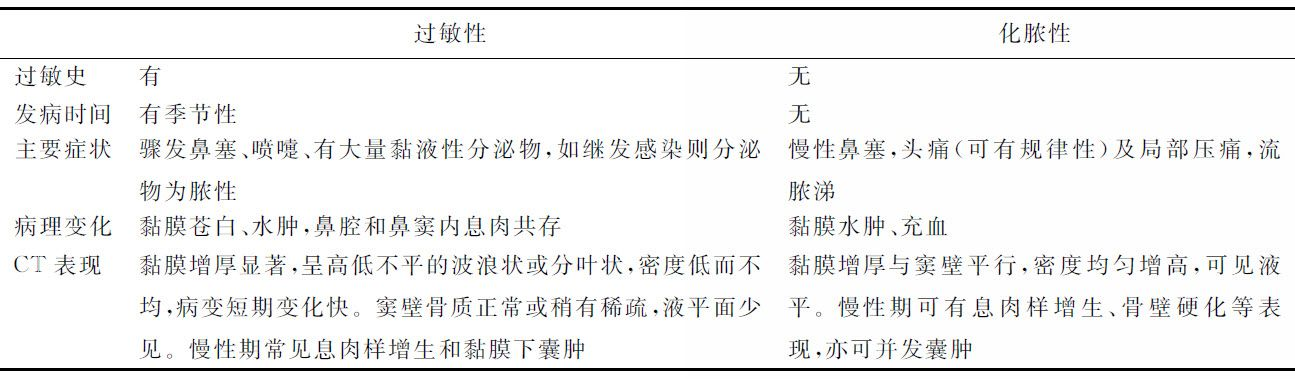
\includegraphics[width=\textwidth,height=\textheight,keepaspectratio]{./images/Image00126.jpg}
\end{table}

\subsection{过敏性鼻旁窦炎}

本病又称为变应性鼻旁窦炎。变态反应为机体一种免疫性保护反应,鼻腔和鼻窦黏膜为变态反应的好发部位。

\textbf{【病因病理】}
引起过敏反应的(变态反应)原因很多,有时难以查明,有的为季节性发作,有的常年发作。有的可伴其他部位的过敏反应。在鼻部主要引起黏膜间质水肿、浆液腺分泌增多。急性发作后可自行消退,如反复发作转为慢性,可使黏膜息肉样肥厚、息肉增生,或腺体阻塞形成囊肿。由于窦口易被阻塞致继发感染,故常合并化脓性炎症。

\textbf{【临床表现】}
主要表现为骤发鼻塞、喷嚏、有大量黏液性分泌物,如继发感染则分泌物为脓性。鼻腔黏膜水肿苍白,有的可伴发息肉。

\textbf{【CT表现】}
多为双侧对称发病。双侧下鼻甲肿胀,鼻窦黏膜增厚显著,呈高低不平的波浪状或分叶状(此表现较化脓性多见),密度低而不均,病变短期变化快。窦壁骨质正常或稍有稀疏。窦腔内积液少见,故液平面少见。慢性期常见息肉样增生和黏膜下囊肿。

\subsection{鼻腔和鼻旁窦息肉}

息肉好发于筛窦和中鼻道,少数可来自中鼻甲下缘、下鼻甲后端、上颌窦等。多数为双侧多发性,单侧少见。

\textbf{【病因病理】}
多认为由变态反应或慢性鼻旁窦炎脓性分泌物长期刺激所致。发生于上颌窦的息肉可经上颌窦口伸展到后鼻孔甚至鼻咽部,称为上颌窦后鼻孔息肉。

一般将息肉分为4类:①鼻息肉伴鼻旁窦炎:最为常见;②鼻旁窦息肉:少见;③鼻旁窦和后鼻孔息肉:多为单侧发生,起源于上颌窦常见,亦可来自蝶窦;④出血坏死性息肉:亦称出血性坏死性上颌窦炎,最常见于上颌窦。

\textbf{【临床表现】}
主要为持续性鼻塞、嗅觉减退、头痛、闭塞性鼻音,常合并鼻旁窦炎。后鼻孔息肉可致呼吸困难。

\textbf{【CT表现】}
①息肉多为水肿型,故呈低密度且无强化的软组织影,慢性增生性息肉内有较明显的炎症和血管增生,密度可较高,且可有强化表现。息肉多位于鼻腔上部的中鼻道,可致鼻中隔偏移、单侧或双侧梨状孔膨大变形,亦可到达鼻前庭和鼻咽部(图\ref{fig5-5})。②鼻腔息肉多伴鼻旁窦阻塞性炎症。③筛窦息肉常为多发,可引起筛小房扩大、小房间隔吸收破坏。④上颌窦息肉可为单发或多发,位于任何部位。⑤上颌窦和蝶窦的息肉可经扩大的自然窦口伸展到后鼻孔、鼻咽部,尤以上颌窦多见。局部有软组织影,且可见窦口扩大伴骨质吸收破坏。

\begin{figure}[!htbp]
 \centering
 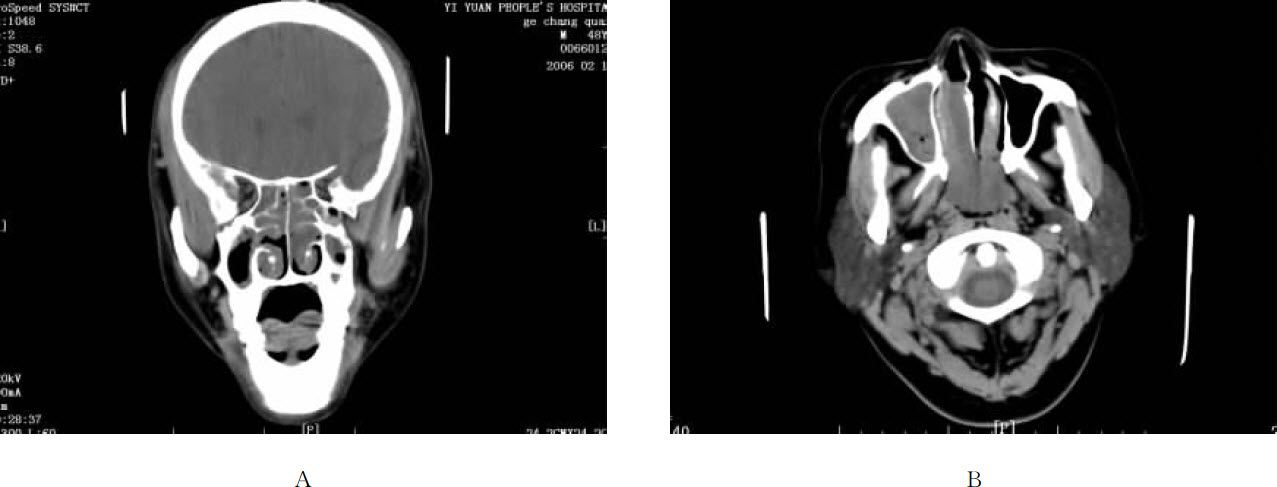
\includegraphics[width=.7\textwidth,height=\textheight,keepaspectratio]{./images/Image00127.jpg}
 \captionsetup{justification=centering}
 \caption{鼻腔息肉并鼻旁窦炎\\{\small A、B非同一患者。A示左右鼻腔内有大量软组织密度灶,充填于各鼻道;左右侧上颌窦、筛窦黏膜显著增厚。B示左右鼻腔内有大量软组织密度灶,密度较低,向后伸展至鼻咽部;右侧上颌窦密实}}
 \label{fig5-5}
  \end{figure} 

\textbf{【鉴别诊断】}

1.鼻旁窦黏膜下或黏液腺囊肿:此类囊肿可发生于任何窦腔的各个部位,一般以上颌窦多见。囊肿小,可多发,但不充满窦腔,常难与窦内小息肉区别。

2.乳头状瘤:鉴别较困难。一般广基、弥漫性生长,肿块中等密度,有强化;而息肉一般不强化,且为低密度。但慢性增生性息肉与肌肉密度相近或稍高且有强化,有时与乳头状瘤等肿瘤难以鉴别;但息肉引起的骨质破坏多为压迫性,有膨胀移位,软组织肿块边缘光滑,与恶性肿瘤之浸润生长和破坏不同。

3.鼻内脑膜脑膨出:可被误认为息肉,但此病出生后即存在,鼻根部可见肿块,穿刺可抽出脑脊液。

4.鼻咽纤维血管瘤:CT特点为位于鼻后孔处强化显著的软组织肿块。

5.恶性肿瘤:软组织肿块强化较明显,骨质呈不规则溶骨性破坏,窦腔无膨大,肿瘤向周围浸润,界限不清(图\ref{fig5-6})。

\begin{figure}[!htbp]
 \centering
 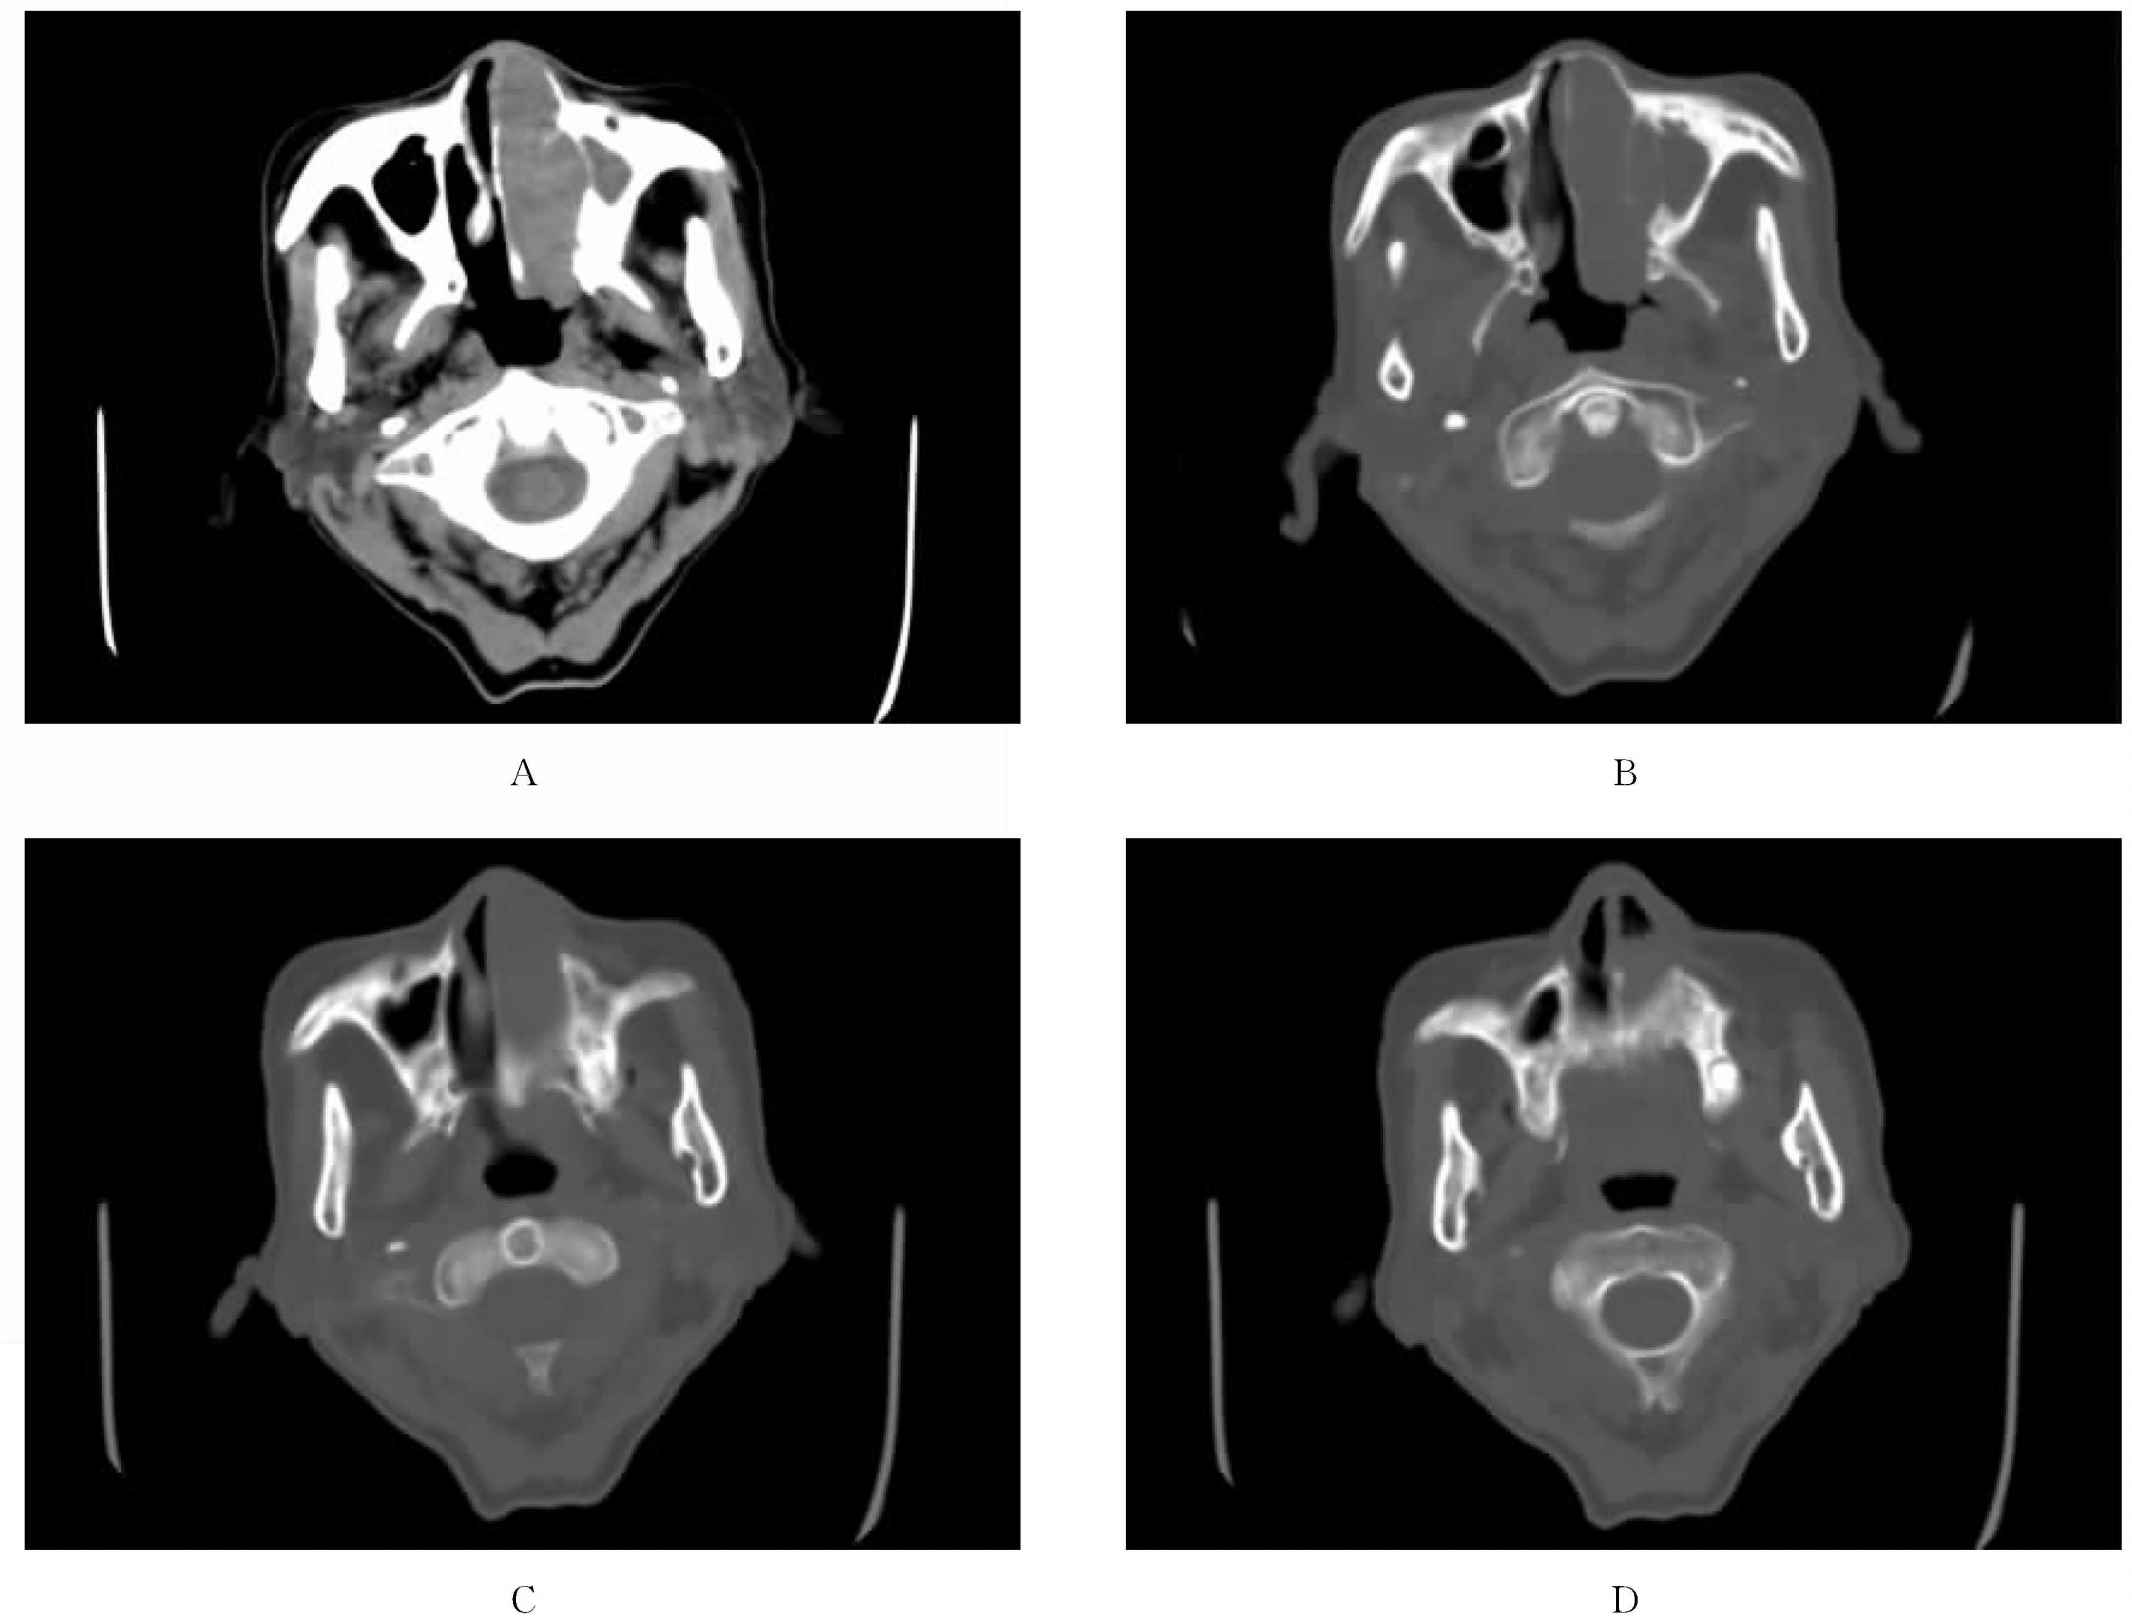
\includegraphics[width=.7\textwidth,height=\textheight,keepaspectratio]{./images/Image00128.jpg}
 \captionsetup{justification=centering}
 \caption{左侧鼻腔恶性黑色素瘤\\{\small 左侧鼻腔内有大量软组织密度灶充填,骨质破坏不明显,与鼻腔息肉不易鉴别}}
 \label{fig5-6}
  \end{figure} 

\subsection{坏死性上颌窦炎}

本病又称出血坏死性上颌窦炎、血管瘤、出血性息肉、血管瘤样息肉。目前大多认为它不同于一般血管瘤而与息肉和炎症关系密切,是上颌窦炎的一种特殊类型,并非多见。多原发于单侧上颌窦,或由鼻腔原发病发展而来,病程长,易反复。

\textbf{【病理】}
大多均有鼻腔或上颌窦腔内的息肉样改变。其息肉组织内血管分布较为丰富,纤维组织相对较少(为临床反复鼻衄并在手术中出血较多的原因所在)。息肉组织内血管旁出血或其形成的组织积存在上颌窦腔内,由于血液的凝固,形成以出血源为中心的血凝块,逐渐机化并可继发感染造成组织的坏死。

\textbf{【临床表现】}
呈典型的反复感染的发病经过,保守治疗效果不理想。均有间歇性鼻堵,多涕(脓涕)。涕可有臭味、常带血丝。还可有头痛、眼眶痛等症状。

\textbf{【CT表现】}
①窦腔密度的改变:平扫显示窦腔内病变密度不均,低密度的炎性病灶与高密度的斑点、斑片状出血区相互混杂。强化不著。②病侧鼻腔改变:可见软组织增生,约占70%,并与上颌窦内病灶相延续。③病变窦腔大小改变:呈不均匀性膨胀扩大,约占73%,与黏液囊肿普遍性扩大有别。④骨质吸收及破坏:约占59%。压迫性骨吸收首先表现在骨壁较薄的上颌窦内侧壁上部,逐渐向下发展,其他各壁较少受累。

总之,窦腔内增强不明显的软组织肿块,其内有斑点、斑片状出血,可伴窦腔扩大是诊断本病的要点之一。

\textbf{【鉴别诊断】}

1.上颌窦恶性肿瘤:一般发生在40岁以后,以男性多见。病程短、发展快,表现为进行性鼻堵、鼻衄和血涕,有特殊臭味。CT表现窦壁呈广泛溶骨性破坏,代之以致密软组织肿块。一般认为上颌窦壁的骨质破坏,尤其除内侧壁外其他各壁的骨质破坏是诊断上颌窦癌的主要依据。

坏死性上颌窦炎病程长,易反复,常呈典型的上颌窦炎表现。CT常表现窦腔软组织病灶内有斑点、斑片状出血,并多见与之相连的鼻腔内软组织肿块。窦壁破坏常位于上颌窦内侧壁上部,窦腔大小正常或呈不均匀性膨大。

2.化脓性上颌窦炎及良性肿瘤:坏死性上颌窦炎的窦腔膨大伴相应骨质吸收为本病区别于一般炎症的要点。这些征象可见于各种良性肿瘤(如纤维瘤、乳头状瘤、神经鞘瘤等)、肿瘤样病变(如囊肿、息肉)和生长较慢的恶性肿瘤(如囊腺癌等)。但良性肿瘤的软组织肿块多不超过破坏边界。

\subsection{真菌性鼻旁窦炎}

鼻和鼻旁窦的真菌感染相对少见。

\textbf{【病因病理】}
最常见的病原菌为曲霉菌和毛霉菌,其他少见的还有念珠菌、鼻孢子菌、隐球菌、放线菌、芽生菌等,其中曲霉菌较毛霉菌常见。①非侵袭性:包括鼻真菌球和变态反应性真菌性鼻窦炎,多见于身体健康者或有过敏体质者;②侵袭性:见于少数病例,包括急性暴发型和慢性侵袭性真菌性鼻窦炎,常见于免疫功能低下或受损者。现在则多直接分为急性暴发型、慢性侵袭型、真菌球和变态反应性真菌性鼻窦炎4种类型。

\textbf{【临床表现】}
多见于成人,女性多见。临床都表现为慢性非特异性鼻炎、鼻旁窦炎的症状,如鼻塞、流脓涕、涕中带血并有腐臭味。擤出污秽的痂皮、碎屑或绿色胶状分泌物,抗生素治疗无效。急性暴发型临床症状严重,进展快,伴有急性发热。有文献报道慢性侵袭型常以突眼为首发症状,但变应性真菌性鼻窦炎也易侵及眼眶,并可致眼球突出。

\textbf{【CT表现】}
①病变多为单侧性,对侧鼻窦鼻腔正常,典型表现为单个上颌窦病变,可累及同侧鼻腔和其他鼻窦。受累窦腔密度增高,病灶可充满窦腔,也可见窦腔中央残留空气影,还可呈类圆形团块(如真菌球)。病灶密度不均匀,有学者统计CT值平均为72Hu,可强化。窦腔黏膜增厚,窦壁骨质有硬化增白。②病灶内70%~90%可见小团块状、砂粒状、片状钙化灶,钙化由磷酸钙沉积于霉菌丝所致(图\ref{fig5-7})。但也有文献认为侵袭性较少有钙化,即使出现,多提示由非侵袭性转变而来。③鼻窦骨质破坏约占28%,主要见于侵袭性患者,但也可见于变应性真菌性鼻窦炎。可广泛破坏且可向颞下窝、眼眶等处侵犯,与恶性肿瘤不易区分。但变应性真菌性鼻窦炎的窦壁骨质以膨胀、变形、变薄吸收更多见。

\begin{figure}[!htbp]
 \centering
 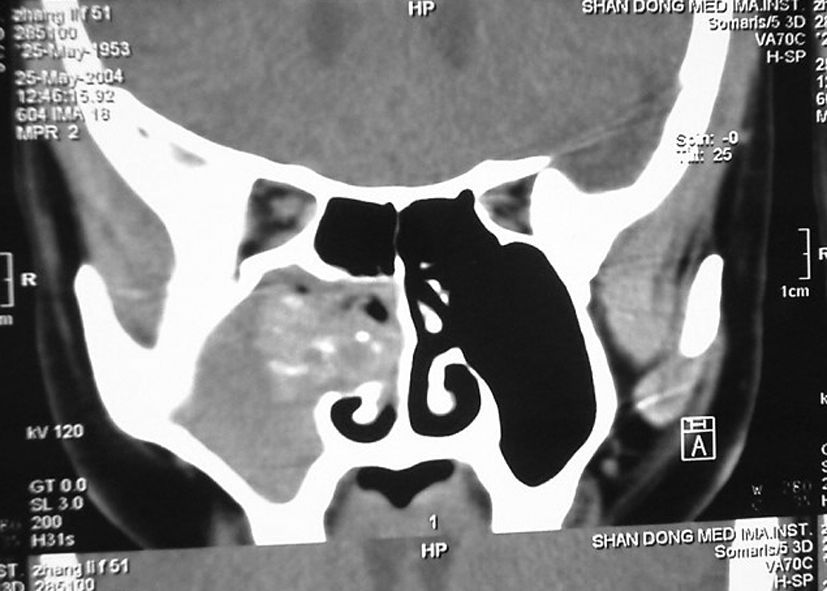
\includegraphics[width=.7\textwidth,height=\textheight,keepaspectratio]{./images/Image00129.jpg}
 \captionsetup{justification=centering}
 \caption{真菌性鼻窦炎\\{\small 右侧上颌窦密实,其内有沙粒状钙化,病灶涉及右侧鼻腔,右上颌窦内侧壁骨质吸收破坏}}
 \label{fig5-7}
  \end{figure} 

\textbf{【鉴别诊断】}

1.化脓性鼻窦炎:多为双侧并累及多个窦腔,可见液平面,无明显骨质破坏,窦壁以增生硬化为主,罕有窦腔内钙化(仅占3%)。窦腔内炎性病灶CT值低,多为30~40Hu。

2.坏死性上颌窦炎:呈增强不明显的软组织肿块,其内有斑点、斑片状出血,可伴窦腔扩大,而无钙化表现,可见上颌窦内侧壁骨质吸收破坏。

3.恶性肿瘤:①如肿瘤比较局限,可见软组织肿块,密度均匀且低于真菌病,CT值多为30~45Hu;②部分肿瘤钙化呈粗大条片状、环状;而真菌病呈小沙砾状、小团状;③恶性肿瘤骨质破坏以溶骨性为主,无明显骨质增生,其形式多样如融雪状、虫蚀状、虚线状或大范围骨质消失,骨破坏区尚可见残存碎骨片;而真菌病骨质破坏局限,多伴骨质增生;④肿瘤有明显的占位效应,窦腔常有明显的扩大;而真菌病窦腔形态改变相对较轻或正常;⑤肿瘤组织向周围侵犯时界限不清;而真菌病向周围蔓延时局限,边界锐利,与脂肪分界清晰。但腺样囊性癌亦可有钙化,且可甚似真菌性鼻窦炎。

\subsection{鼻和鼻旁窦结核}

鼻结核多发生在鼻腔的中隔面,鼻窦结核多发生于上颌窦,由呼吸道、淋巴或血行播散所致。

\textbf{【病理】}
有渗出性和增殖性病变2类。轻者仅侵及皮肤、黏膜和软骨,进而出现溃疡和肉芽肿,较重时可导致骨质破坏,形成慢性脓肿、瘘管或有死骨存在,常伴化脓性感染。

\textbf{【临床表现】}
主要为鼻塞、分泌物增多、鼻衄、流泪,鼻或颊面部肿胀、疼痛,有时还有颈淋巴结肿大。鼻腔检查可见溃疡及肉芽,或有鼻中隔黏膜萎缩。确诊依靠实验室及病理组织学检查。

\textbf{【CT表现】}
鼻结核多显示鼻腔内软组织影增多,骨性鼻中隔可吸收、破坏。上颌窦结核表现为窦腔内软组织密度灶,有或无脓液。不少患者有窦壁骨质破坏、死骨及瘘管形成。骨质破坏典型者多呈稀疏吸收,少有反应性增生。但常继发感染,故硬化现象并不少见。

\subsection{鼻梅毒和雅司病}

鼻部可为第3期梅毒或雅司螺旋体侵犯,于感染后3~10年发病。

\textbf{【病理】}
两者病理改变相似,主要为树胶样肿侵犯邻近组织结构。可侵犯鼻部的皮肤、黏膜、软骨和骨,可导致鼻中隔穿孔、鼻梁塌陷等,常伴化脓性感染。

\textbf{【临床表现】}
早期出现无痛性溃疡,晚期出现鼻塞、流脓涕、恶臭、局部硬质小结节,鼻梁毁坏者呈鞍鼻。血清学检查有定性意义。

\textbf{【CT表现】}
早期显示鼻腔软组织密度灶,鼻窦黏膜增厚。晚期鼻骨和骨性鼻中隔吸收、破坏、消失,鼻窦骨质硬化、增生,破坏较轻。

\subsection{鼻硬结病}

本病是一种少见的慢性进行性肉芽肿,由克雷伯鼻硬结杆菌引起,好发于农民。多见于贫穷、卫生条件差的地方,在我国少数地区(如山东省等)发生。

\textbf{【病理】}
病变通常始发于鼻前庭鳞状上皮与纤毛柱状上皮的结合处,然后沿着黏膜固有层向四处蔓延,可涉及前后鼻孔、咽、喉、硬腭、软腭、气管、鼻窦、口腔,亦可向眼眶扩展。早期有鳞状上皮化生和肉芽组织形成,进而有肉芽肿性结节和纤维瘢痕形成,可使腔道狭窄粘连。病理分为卡他性鼻炎期、肉芽肿期和瘢痕期。

\textbf{【临床表现】}
多见于20~40岁的男性。早期可无症状。后期典型症状有鼻塞、鼻干、鼻臭和失嗅,还可有鼻衄、鼻面部畸形,涉及咽、喉、气管等出现相应症状。

\textbf{【CT表现】}

1.鼻腔硬结病:多两侧对称发病,但极少数为局限性或非对称性。①早期表现为非特异性鼻腔黏膜增厚。②肉芽肿期呈界限清楚的不规则软组织肿块,肿块大小、数目不一,可融合成形态不规则的大肿块;密度均匀,无明显强化。中、下鼻甲和骨性鼻中隔可有吸收破坏,但残存的骨质常明显硬化。可有鼻窦受侵或阻塞性炎症所致的窦腔实变。还可侵犯眼眶甚至颅内,出现脑膜增厚、脑实质肉芽肿。③瘢痕期邻近骨质破坏明显,鼻腔狭窄,鼻腔内黏膜萎缩纤维化而见散在条索影。

2.鼻窦硬结病:常原发于上颌窦,其次为筛窦、蝶窦,额窦罕见,极易误诊为恶性肿瘤。表现为窦腔内不规则软组织肿块,密度均匀,界限清楚,易侵犯邻近结构。窦壁有骨质破坏,但残端和周围骨质明显硬化。

\textbf{【鉴别诊断】}
①萎缩性鼻炎:有鼻干、鼻臭,但多无出血。CT表现为鼻甲萎缩,以下鼻甲最常见。通常无明显软组织影,亦无鼻窦等部位的受侵。②其他:与Wegener肉芽肿、淋巴瘤、鼻窦恶性肿瘤、慢性侵袭性真菌性鼻窦炎可难以鉴别。但鼻硬结病骨质破坏边缘的明显硬化,有一定鉴别价值。

\subsection{鼻旁窦胆固醇肉芽肿}

胆固醇肉芽肿在头面部好发于中耳乳突,鼻旁窦少见,为出血部位析出的胆固醇结晶引起异物反应形成的肉芽肿病变。鼻旁窦内病灶的形成可能与出血和外伤后引流不良有关,多见于上颌窦和额窦。

\textbf{【CT表现】}
病变窦腔内充满近软组织样密度灶;可致窦腔扩大,骨壁压迫性吸收破坏。有的可发生于骨内,以眶上的额骨多见,病灶边缘清,但无硬化。应注意与额骨皮样囊肿相鉴别,后者边缘光滑锐利且有硬化。

MR示胆固醇肉芽肿T\textsubscript{1} 加权和T\textsubscript{2}
加权均呈高信号,比CT有定性意义。

\subsection{巨细胞修复性肉芽肿}

发生于鼻和颌面部的巨细胞破坏性病变较少见,有巨细胞修复性肉芽肿、甲状旁腺功能亢进引起的骨膜下吸收的棕色瘤和真正的巨细胞瘤等。它们的组织学和影像学表现常相似,应结合临床和病理进行诊断。

\textbf{【病理】}
巨细胞修复性肉芽肿为发生在颌面骨、蝶骨和颞骨(亦有发生于岩锥的报道)等部位的巨细胞破坏性病变。肿块无包膜,病灶内为富血管的肉芽组织所组成,其中有斑块状的骨样组织沉积和反应性新骨形成,可伴有出血和囊变。组织学上可见梭形细胞基质中含有多核巨细胞。

\textbf{【临床表现】}
好发于青壮年,25岁以上占86%,多数有外伤、感染史。瘤样病变多是出血或创伤的炎症修复性反应,伴有局部疼痛和触痛。

\textbf{【CT表现】}
骨膨胀性破坏及软组织肿块影,可伴瘤内出血及骨化,增强扫描可有强化。部分界限清楚,骨质破坏多较显著,少有隔。

\subsection{鼻和鼻窦坏死性肉芽肿}

本病又称恶性肉芽肿、致死性中线肉芽肿、不愈合性肉芽肿等。为一少见的进行性坏死性溃疡,伴有非特异性肉芽组织增生,可合并感染。

\textbf{【病理】}
大多认为病理分型有局部病变和系统性病变之分,两者在病理和临床上有所不同。①局部型:又称为肿瘤型、Stewart型或面中线致死性肉芽肿。好发于鼻、面和咽腭部,呈多发性溃疡和进行性破坏;病理上为非特殊性急、慢性炎症,肉芽肿内有多形细胞(以淋巴细胞为主)浸润,有人认为属恶性淋巴瘤的一种类型。②全身型:又称为Wegener型。除鼻、咽、喉等上呼吸道病变外,还有肺、肾、脾和淋巴结等全身器官受累;病理上以坏死性血管炎和血管周围炎为特征,其内含有多核巨细胞;大多认为属免疫性病变。

\textbf{【临床表现】}
可发病于任何年龄,以青壮年多见。常见鼻、面、口腔和咽部黏膜溃烂、组织坏死,甚至可侵犯眼眶。全身症状有发热、肺炎、肾炎、关节炎等,最终死于恶病质、肾衰、出血和感染。

\textbf{【CT表现】}
多无特征性,早期表现类似一般鼻炎和鼻旁窦炎。鼻腔、面部、口咽部软组织肿胀增厚,鼻旁窦内黏膜增厚。进一步发展可破坏软组织、软骨和骨,并可涉及鼻中隔、上颌骨、腭骨甚至筛窦、额窦和蝶窦。

\textbf{【鉴别诊断】}
①骨破坏区多不伴有软组织肿块,而恶性肿瘤的骨破坏区常伴软组织肿块影,可以鉴别。②咽部病变与早期鼻咽癌和炎症区别困难,需靠组织学诊断。③结节病形成的肉芽肿可以充满鼻旁窦腔并使窦壁膨胀,与本病、淋巴瘤等恶性肿瘤相似,应注意鉴别。

\subsection{鼻旁窦黏液囊肿}

本病是鼻旁窦中最常见的膨胀性病变,是由于鼻旁窦开口阻塞后窦内黏液潴积所致。

\textbf{【病因病理】}
窦口阻塞的原因有:①慢性炎性病变:如息肉、黏液腺囊肿;②外伤和手术后骨质增生或瘢痕封闭;③良、恶性肿瘤阻塞;④解剖变异。囊肿的壁为鼻旁窦壁黏膜,可增厚、息肉样变或纤维化。内容物呈淡黄色、棕褐色或暗绿色的黏稠液体,内含大量胆固醇;如有感染则变为脓性液体,称为脓囊肿。囊肿很大时,可使窦壁变薄或破坏,并可向眶内或颅内发展。

\textbf{【临床表现】}
一般发展缓慢,常向窦周膨隆致眼球突出和移位、局部隆起或可扪及软性肿块,有的可有局部疼痛、视力减退及眼球运动障碍。继发感染可有全身症状如发热、头痛、全身不适等,局部表现红肿、压痛。

\textbf{【CT表现】}
本病好发于额窦和筛窦,其次为蝶窦,上颌窦相对少见。多单个窦腔发生,但亦可发生于两个邻近鼻旁窦。平扫表现为窦腔内软组织密度影,边缘光滑呈弧形,可见均匀细薄的稍高密度的囊壁。当囊肿呈高压时,窦腔呈类圆形膨胀性扩大变形,窦壁呈弧形变薄或外移,是窦内良性占位的重要征象。增强扫描囊内液体不强化,CT值约20Hu左右,囊壁有线形强化,合并感染者囊壁增厚。窦壁骨质可变薄、吸收。由于囊肿常合并有慢性炎症,故窦壁硬化增白亦常见。有时可见窦口阻塞的原因,囊肿侵及眼眶、颅内可出现相应的表现。

\subsection{鼻旁窦黏膜下囊肿和黏液腺囊肿}

两者统称为黏膜囊肿。关于两者的命名国内有关专著有混淆现象,其影像学表现类似。常见于上颌窦,额、蝶窦次之。平时无症状,常意外发现,偶有头痛,有时囊肿自行破裂从鼻腔中流出黄色液体。

\subsubsection{黏膜下囊肿}

又称浆液囊肿或潴留囊肿,是含蛋白的液体潴留于黏膜下的疏松结缔组织中而形成,其囊壁为结缔组织而无上皮组织,实际上并非真正囊肿,其发生可能与变态反应或慢性炎症有关。

\textbf{【CT表现】}
囊肿多为单窦单发,亦可单窦多发、多窦单发或多窦多发,但少见。多位于窦腔基底部,呈半月形或类圆形中等密度软组织肿块,边缘光滑,密度均匀,增强扫描囊肿无强化。大的可占满整个窦腔,窦腔膨大和骨质吸收远较黏液囊肿少见,程度较轻(图\ref{fig5-8})。

\begin{figure}[!htbp]
 \centering
 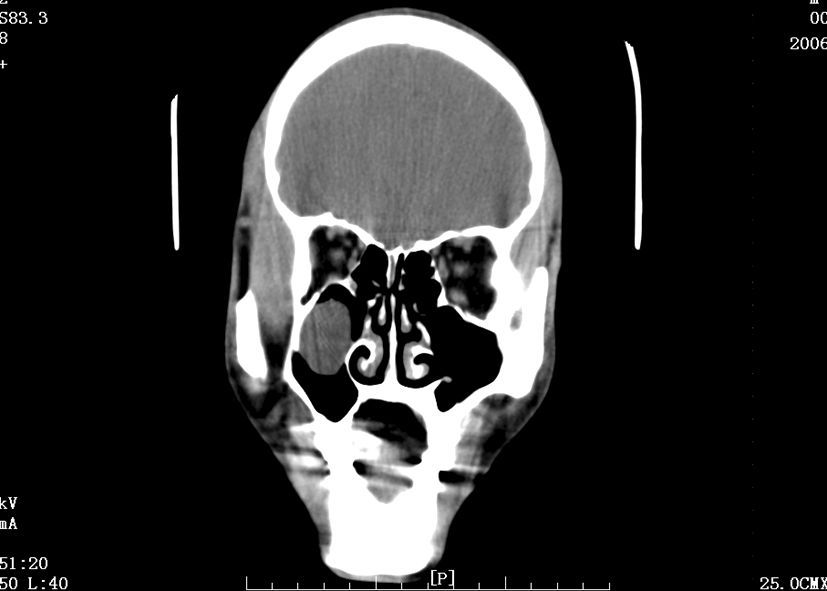
\includegraphics[width=.7\textwidth,height=\textheight,keepaspectratio]{./images/Image00130.jpg}
 \captionsetup{justification=centering}
 \caption{右侧上颌窦囊肿\\{\small 右侧上颌窦腔内有类圆形中等密度软组织肿块,边缘光滑,密度均匀}}
 \label{fig5-8}
  \end{figure} 

\subsubsection{黏液腺囊肿}

为窦内黏液腺管口阻塞,引起腺管内黏液滞留而成,故囊壁为黏液腺管之上皮,很少长得很大,一般无症状。

\textbf{【CT表现】} 与黏膜下囊肿相类似,两者难以区分。

\subsection{鼻窦气囊肿}

\textbf{【病因病理】}
本病发病机制尚不清楚,可能为窦口呈活瓣性阻塞即气体易进难出所致。有人认为可能为窦内囊肿形成后,使窦壁吸收变薄,以后窦口恢复引流,囊肿破裂液体排空,窦口外形成单向阻塞,空气只进不出,长时间后形成含气囊肿。气囊肿壁为鼻窦黏膜。

\textbf{【CT表现】} 窦腔扩大,窦壁有膨胀表现,其内为气体密度。

\section{肿瘤}

\subsection{概述}

\subsubsection{鼻腔和鼻旁窦良、恶性肿瘤的分类}

1.良性肿瘤:较少见,但组织学种类较多。主要有乳头状瘤、混合瘤、血管瘤、出血性息肉、神经鞘瘤、骨瘤、骨化性纤维瘤、软骨瘤、骨软骨瘤、骨纤维异常增殖症、巨细胞瘤、脑膜瘤(可原发)等。

2.恶性肿瘤:相对较多见,占耳鼻喉科恶性肿瘤的25%~50%。发生率依次为鼻腔、上颌窦、筛窦、额窦和蝶窦。主要有:①起源于上皮的鳞状细胞癌、未分化癌、腺癌、腺样囊性癌、黑色素瘤;②起源于间质的肉瘤,如淋巴瘤、浆细胞瘤、恶性纤维组织细胞瘤、网织细胞肉瘤、嗅神经母细胞瘤、纤维肉瘤、平滑肌肉瘤、脂肪肉瘤、软骨肉瘤、成骨肉瘤、恶性巨细胞瘤、横纹肌肉瘤、血管母细胞瘤、混合瘤恶变等。其中,以鳞状细胞癌最为多见。

此外,良性肿瘤也有恶变的,如鼻息肉恶变、乳头状瘤恶变、纤维瘤恶变为纤维肉瘤等。

\subsubsection{鼻腔肿物的诊断原则}

一般情况是,根据肿块的轮廓是否光整用以区别良、恶性,但鼻腔良性病变中的乳头状瘤和肉芽肿等亦可出现凹凸不规则的边缘,导致诊断上的困难。良性肿物一般不引起骨质破坏,但少数病例肿物较大或合并感染时,可呈现鼻中隔和(或)鼻腔侧壁破坏,酷似恶性肿瘤。但如显示鼻腔侧壁变薄,呈弧形外凸和鼻中隔推移等膨胀性改变较明显时,仍应考虑为良性肿物。

鼻腔恶性肿瘤一般无鼻中隔移位和鼻腔扩大变形,鼻腔侧壁和鼻中隔可见骨质吸收或不规则破坏,肿瘤同侧鼻窦密度增高,但少数局限于鼻腔的恶性肿瘤可无骨破坏。晚期邻近上颌窦、筛窦、眶骨等可出现不规则骨质破坏。

此外,应注意鼻腔鼻窦解剖结构与眼眶、口腔、颌面骨及鼻咽部关系密切,这些部位的肿瘤互相侵犯,影像学有时难以确定其来源,需密切结合临床资料综合分析。

\subsubsection{鼻窦良、恶性肿瘤的诊断原则}

1.良性肿瘤:较少见,好发于青年人,以骨瘤较常见。良性肿瘤常导致窦腔扩大、膨胀变圆,窦壁可以完整;如肿瘤较大,可导致骨质压迫性吸收及破坏,但进展缓慢,常隐约可见部分骨结构存留。①骨瘤:好发于额窦内,筛窦次之,偶可窦外生长;亦可分为密质型、松质型和混合型3类。②骨软骨瘤:见斑点状钙化分布于整个肿块表面。③骨化性纤维瘤:瘤体呈高密度不均匀的骨化肿块或包壳厚而不均且有斑点状骨化影为其特征。④骨内血管瘤:以蜂窝状破坏较为典型,增强扫描血管瘤显著强化有别于神经鞘瘤等。

总之,CT能全面显示良性肿瘤所特有的软组织增生、窦腔扩大变形或骨壁呈边缘锐利的缺损等表现。

2.恶性肿瘤:鼻窦肿瘤以恶性居多,主要为癌肿和肉瘤。癌肿好发于成年人和老年人,肉瘤多见于青年人,鼻腔鼻窦横纹肌肉瘤多见于婴儿和儿童。①恶性肿瘤一般不引起窦腔扩大,主要表现为软组织肿块及骨质侵蚀破坏,进展较快,骨破坏多较完全或边缘不规则。②少数低度恶性肿瘤和肉瘤有时也可见轻度窦腔扩大,但多有较明显的骨质破坏伴随。③骨肉瘤有溶骨型、硬化型和混合型之分,有时可见垂直外表的放射状骨针。④软骨肉瘤以骨质破坏为主,有时破坏区之软组织肿块中可见高密度钙化影,且无强化或强化不著,有别于其他恶性肿瘤。⑤CT扫描可清楚的显示向窦周的侵犯情况。

但应注意以下情况:①少数局限于鼻窦的恶性肿瘤可无骨质破坏,故无明显骨质破坏不能除外肿瘤存在。②骨质破坏并非恶性肿瘤所特有,如真菌病和坏死性上颌窦炎也可发生。真菌病如无钙化、坏死性上颌窦炎如无出血则与恶性肿瘤鉴别困难。③少数恶性肿瘤(如乳头状瘤恶变、黏液上皮癌、上颌窦腺样囊性癌以及某些肉瘤)也可引起窦腔扩大,与良性肿瘤相似。但一般恶性肿瘤破坏程度多比窦腔扩大更显著有助鉴别,亦可难以判断。④骨和软骨类肿瘤可有钙化和骨样结构,不同于上皮癌肿,但其良恶性或恶变难由影像学检查作出准确判断。⑤不少恶性肿瘤伴有鼻旁窦炎症,辨别肿瘤侵犯范围颇为重要。骨质破坏为肿瘤侵犯的重要依据,增强后肿瘤也较炎症组织密度高,可助鉴别。MR一般显示肿瘤较炎症信号低。⑥鼻窦转移瘤罕见,如肾癌、乳癌、肺癌甚至胃肠道癌可转移到鼻窦。

\subsubsection{鼻腔和鼻旁窦肿瘤的影像学定性诊断原则}

虽然CT和MR分辨率高,但定性价值有限,定性诊断仍以形态学为基础。①类圆形的膨胀性肿块多见于良性肿瘤或囊肿;少数也可见于生长较慢的低度恶性肿瘤或较大的肉瘤;②形态不规则的软组织增生多见于肿瘤和肉芽肿性病变;③良性肿瘤和囊肿边缘多较光滑和清楚;恶性肿瘤和炎症可为浸润性,边缘欠清晰;④良性膨胀性病变可致窦腔扩大和骨壁压迫性吸收;恶性肿瘤和肉芽肿则以窦壁侵蚀性破坏或伴窦外软组织浸润增生为要点;⑤囊肿一般为均质低密度(CT)或均质高信号(MR);⑥炎症和肿瘤均可有强化;⑦肿瘤内密度多为混杂不均;⑧钙化和骨化为某些病变的特点。

总之,综合影像和临床可做初步定性诊断,病理组织学仍为确诊的主要方法。

\subsection{鼻腔及鼻旁窦乳头状瘤}

本病是鼻腔及鼻旁窦较常见的良性上皮肿瘤,肿瘤的组织形态介于癌组织与正常上皮之间。病因不明,有术后复发和恶变的倾向。

\textbf{【病理】}
可分为两型:①内翻型乳头状瘤:多见,且易术后复发和恶变。好发于鼻腔侧壁,常侵入筛窦和上颌窦,主要由移行上皮细胞和柱状上皮细胞增殖形成。病理特点为上皮成分向基底内呈内翻性生长,基底膜水肿,呈息肉状肿块。②外生型乳头状瘤:少见,外观似疣状。好发于鼻中隔前部或鼻前庭,主要由鳞状上皮细胞增生组成。术后少见复发,极少恶变。

\textbf{【临床表现】}
多见于40岁以上,50~60岁发病率高,男多于女。常以鼻塞和鼻出血就诊,鼻腔内可见息肉状肿块,可误认为鼻息肉。筛窦、上颌窦受侵者可致眶面部变形。

\textbf{【CT表现】}
缺乏特征性,鼻腔和鼻旁窦内充满较高密度的软组织影,边缘清楚,呈不规则结节状,增强扫描呈中度均匀强化。内翻乳头状瘤可向后扩展至后鼻孔、鼻咽部。鼻旁窦乳头状瘤可引起窦腔的扩大、筛房间隔和上颌窦壁吸收破坏;鼻腔内病灶可使鼻甲及上颌窦内侧壁骨质吸收变薄(图\ref{fig5-9})。

\begin{figure}[!htbp]
 \centering
 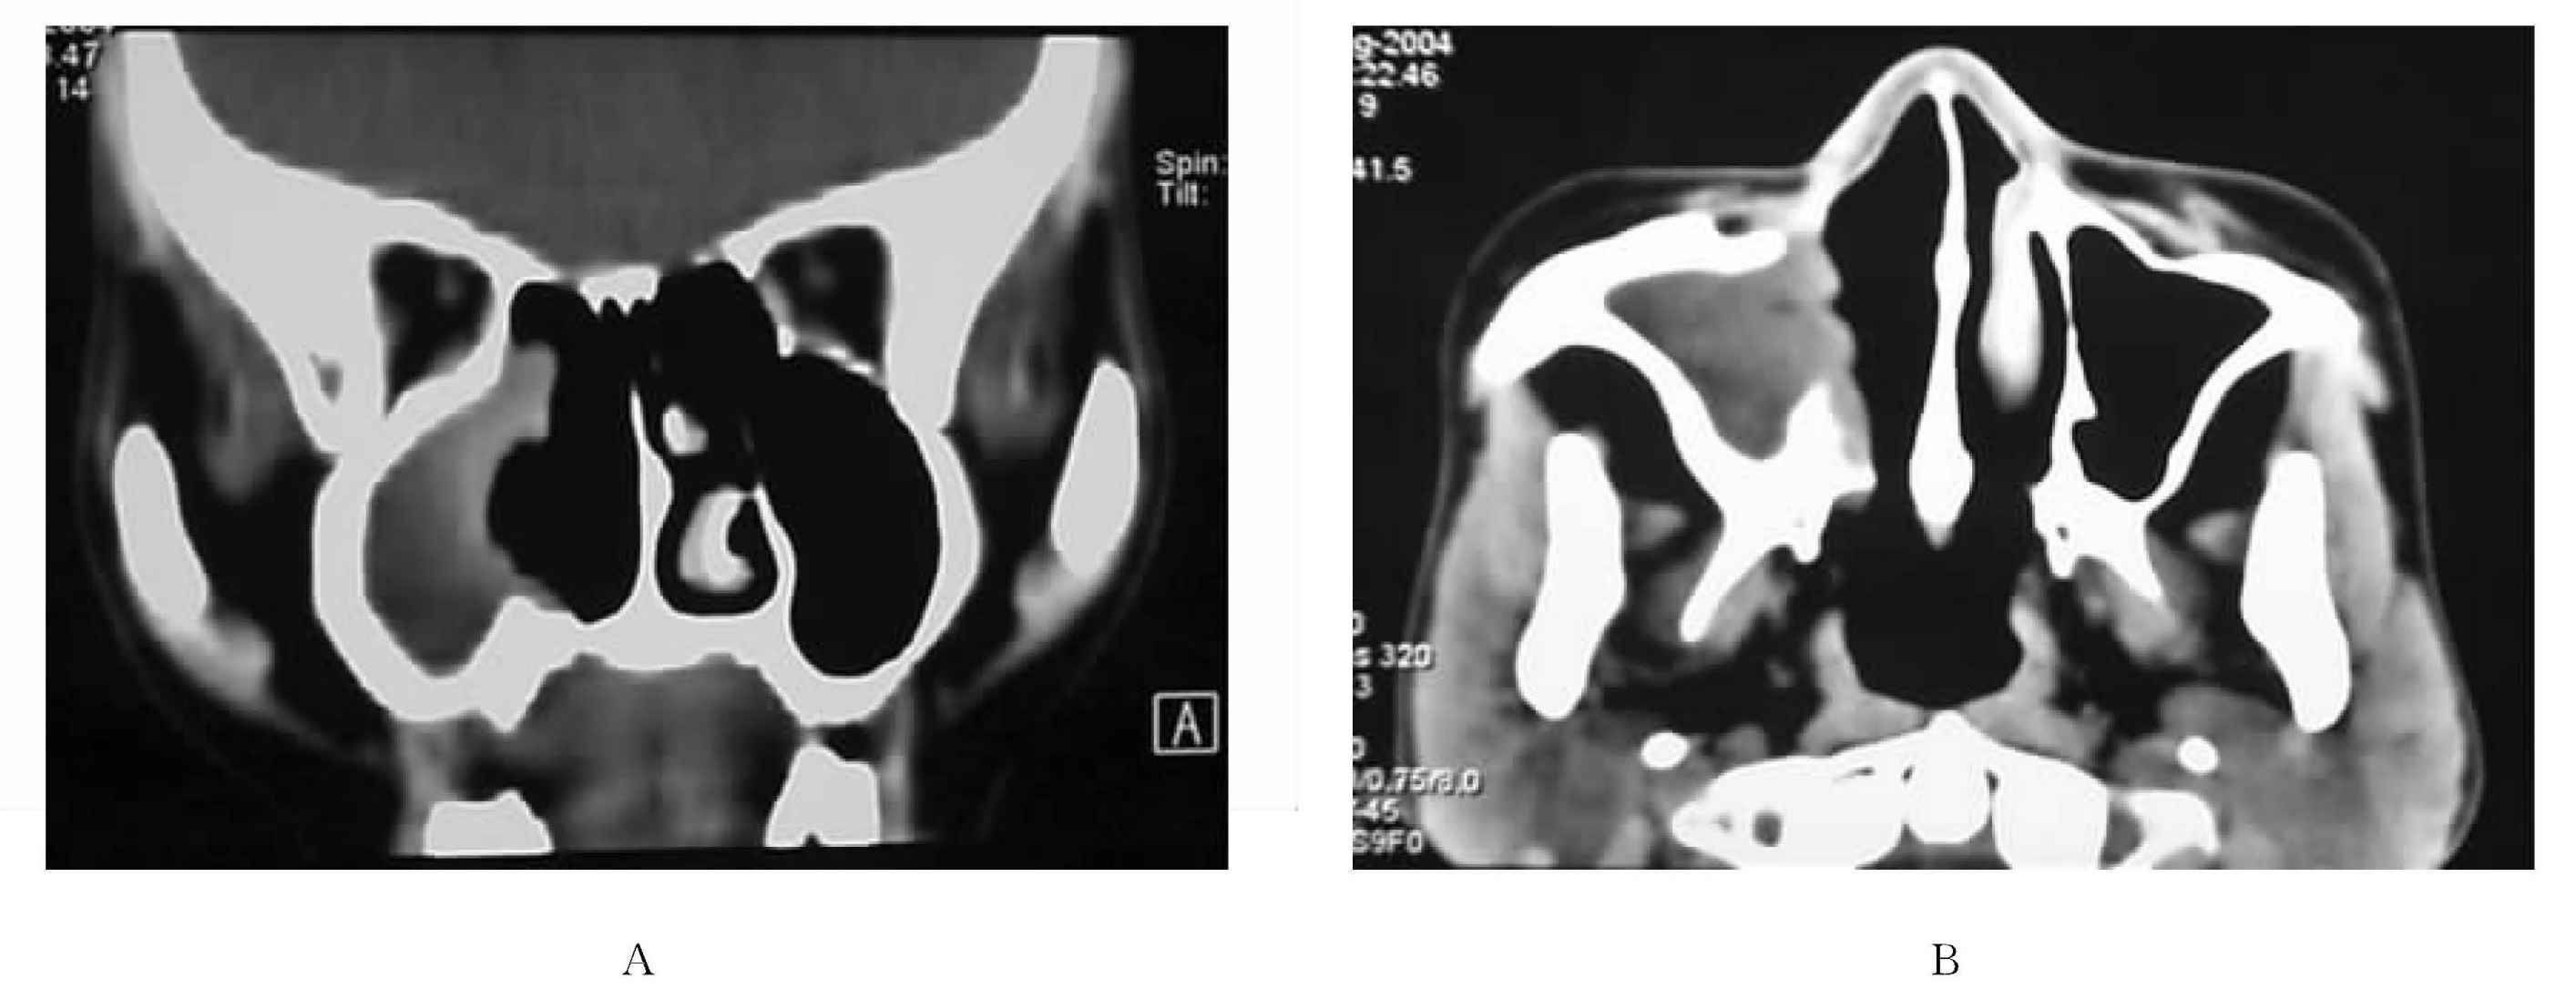
\includegraphics[width=.7\textwidth,height=\textheight,keepaspectratio]{./images/Image00131.jpg}
 \captionsetup{justification=centering}
 \caption{鼻内翻乳头状瘤\\{\small 右侧上颌窦内有软组织肿块,内侧壁骨质吸收破坏}}
 \label{fig5-9}
  \end{figure} 

\textbf{【鉴别诊断】}
①息肉:好发于中鼻道,一般呈类圆形结节,多为低密度,不强化。②出血坏死性上颌窦炎:呈高低混杂密度,骨质破坏不如乳头状瘤明显,但鉴别有时困难。③恶性肿瘤:呈强化明显的软组织肿块,浸润性生长,骨质破坏范围广,向周围组织浸润,边界不清。

\subsection{骨瘤}

本病为最常见的鼻窦良性肿瘤,生长缓慢、可有自行停止生长的趋势。

\textbf{【病理】}
基本发生于鼻窦的骨壁上,通常单发,带蒂或基底宽,上颌窦、蝶窦少见。一般分为3型:即密质型(多见于额窦)、松质型(多见于筛窦)和混合型(多见于额窦)。

\textbf{【临床表现】}
多见于20~40岁成人,大多无症状,大者可引起鼻窦阻塞症状,甚至引起黏液囊肿。

\textbf{【CT表现】}
圆形或分叶状致密骨块,小者数毫米,大者可充满窦腔。密质型密度均匀致密;松质型边缘有细薄的骨皮质,瘤内可见均匀致密的骨小梁;混合型为纤维骨瘤,高密度的瘤体内夹杂有较多的低密度成分。

\subsection{骨化性纤维瘤}

本病是一种良性的纤维骨性疾病,好发于上颌骨、额骨、筛骨、蝶骨和颞骨等。通常认为不恶变,但也有文献认为0.4%会发生恶变。

\textbf{【病理】}
多为单发,大小不一,基底宽。有包膜,边界多清楚。镜下多由梭形成纤维细胞和致密骨组织组成,骨小梁周边可见成骨细胞。瘤体可有囊性变。

\textbf{【临床表现】}
本病可有两个发病高峰,青少年和30~40岁,女性多于男性。早期可见面颊部无痛性肿胀、鼻塞和感觉异常;较大者侵入眼眶、颅底,可出现视力障碍、眼球移位等症状。

\textbf{【CT表现】}
呈椭圆形高密度肿块,可有分叶,边缘清楚,范围局限。瘤体周壁和肿块内可见钙化和骨化,壁厚而不均,有占位效应,可有囊变区。被侵犯的鼻窦腔可膨大变形,侵及眼眶或颅底表现为膨胀压迫改变。增强扫描部分瘤体实质有强化。

\subsection{骨纤维异常增殖症}

本病是一种原因不明的以骨内纤维异常增生为特征的骨疾病,为自限性的良性病变,好发于上颌、蝶骨、额骨。

\textbf{【病理】}
病变区骨组织被坚韧的纤维组织所代替,局部骨皮质膨胀变薄或侵蚀。病灶主要由不同成熟程度的纤维组织和新生的不成熟的骨样组织所构成。可分为单骨型、多骨型和多骨型伴内分泌紊乱3种类型。

\textbf{【临床表现】}
病变进展缓慢,一般幼年发病,长大后产生症状。病变部位畸形肿胀,可有眼球突出、鼻塞、鼻腔狭窄、牙齿松动等。侵及颅神经可产生相应颅神经受损的症状和体征。

\textbf{【CT表现】}
病变可呈磨玻璃状、致密骨样和囊性变,常混合存在。骨密度多均匀增高,受累的骨体增大变厚,界限欠清,可有包壳,鼻窦腔缩小。

\subsection{血管瘤}

鼻部毛细血管瘤多位于鼻中隔;海绵状血管瘤多位于鼻甲、外鼻,偶见于鼻旁窦或邻近面颅骨。

\textbf{【病理】}
根据临床和组织结构特征一般分为毛细血管瘤、海绵状血管瘤和蔓状血管瘤。毛细血管瘤较小,可有蒂;海绵状血管瘤较大而基底广,由大小不等的血窦组成。

\textbf{【临床表现】}
单侧进行性鼻阻塞、反复鼻出血为其主要表现,鼻腔内可见紫红色肿块。肿瘤大者可自梨状孔脱出或向后进入鼻咽部。

\textbf{【CT表现】}
鼻腔和(或)鼻窦内形状不一的软组织肿块,边缘光滑、锐利,增强扫描显著强化。偶见静脉石具有特征性,局部骨质可受压变形、吸收破坏。鼻窦或面颅骨内蜂窝状破坏有一定特征,有的肿瘤可向软组织内生长伴骨膜骨质增生。

\subsection{神经源性肿瘤}

神经鞘瘤和神经纤维瘤均可发生于鼻腔和鼻旁窦,但极少见。

\textbf{【临床表现】}
常表现为鼻塞、鼻出血、疼痛、流涕、复视、突眼等症状。

\textbf{【CT表现】}
膨胀性、类圆形肿块,边缘光滑(有包膜),密度多均匀,但神经鞘瘤可有囊变而致密度不均。增强扫描多强化,肿瘤偶有钙化。窦腔和鼻旁窦扩大,部分有骨质破坏。

\subsection{上颌窦恶性肿瘤}

上颌窦恶性肿瘤的发病率占各个鼻旁窦之首(80%),占全身恶性肿瘤的1%~2%,占耳鼻喉科恶性肿瘤的20%,仅次于鼻咽癌,居第二位。

\textbf{【病理】}
多为原发,转移性罕见,但一小部分来自邻近器官。主要以鳞癌多见(80%),腺癌次之,其他上皮癌和肉瘤等均少见。肿瘤早期常局限于窦腔,随发展占据整个窦腔,进而向邻近组织器官浸润蔓延。

\textbf{【临床表现】}
本病男性多见,男女之比约4∶1。癌肿多见于50岁左右,肉瘤多见于30岁以下。早期局限于窦腔可无症状,偶有血涕。随病变进展可出现面颊部疼痛、麻木,牙痛、松动,流脓血涕、鼻阻塞,面部鼻部畸形,复视、突眼等。可触及转移肿大的颈部淋巴结。

\textbf{【CT表现】}
①上颌窦鳞癌的特征性表现是窦腔软组织肿块并骨质破坏,部分肿瘤钙化呈粗大条片状、环状。增强扫描肿瘤有强化。上颌窦广泛性骨质破坏,以溶骨性为主,无明显骨质增生,其形式多样如融雪状、虫蚀状、虚线状等(图\ref{fig5-10})。一般认为上颌窦壁的骨质破坏,尤其除内侧壁外其他各壁的骨质破坏是诊断上颌窦癌的主要依据。②上颌窦肉瘤与癌肿类似,可有低密度坏死或囊变区;骨肉瘤有排列紊乱、无正常骨结构的高密度瘤骨。

\begin{figure}[!htbp]
 \centering
 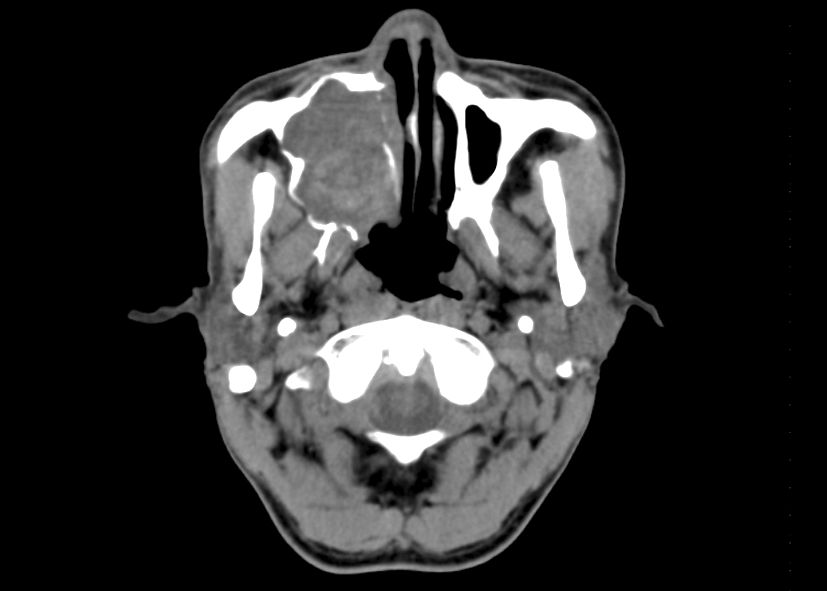
\includegraphics[width=.7\textwidth,height=\textheight,keepaspectratio]{./images/Image00132.jpg}
 \captionsetup{justification=centering}
 \caption{右侧上颌窦癌\\{\small 右侧上颌窦腔内软组织肿块合并较广泛骨质破坏}}
 \label{fig5-10}
  \end{figure} 

\textbf{【鉴别诊断】}
①上颌窦黏膜息肉样变:单纯黏膜改变,尤其是早期癌变与其很难区分。肿瘤可有局部窦壁的骨吸收及破坏,而炎性息肉常为窦壁增厚硬化。②出血坏死性上颌窦炎:主要为上颌窦内充满软组织,且软组织内有不均匀较高密度的出血斑块。窦腔可有膨胀性改变,窦自然开口有扩大,鼻腔内有类似软组织肿块。③真菌性鼻窦炎(见本章第五节)。④乳头状瘤:临床上病史较长,与恶性肿瘤常难以鉴别,有时需行活检鉴别。

\subsection{筛窦恶性肿瘤}

在鼻窦恶性肿瘤中,筛窦恶性肿瘤发病率仅次于上颌窦。

\textbf{【病理】}
原发者少见,多继发于鼻腔、上颌窦的恶性肿瘤,少数也可来自泪囊、眼眶、鼻咽、蝶窦等部位的恶性肿瘤。主要以鳞癌多见,其他有腺癌、腺样囊性癌和各种肉瘤。

\textbf{【临床表现】}
本病男性远多于女性,主要表现为涕血、鼻塞、鼻顶塌陷等,也可无鼻内异常。常可涉及眼眶表现为突眼、复视、泪溢、眼球运动和视力障碍等。侵入颅内或颅神经出现头痛及颅神经受损的症状。

\textbf{【CT表现】}
原发者表现为筛窦内局部软组织肿块伴有筛骨纸板、筛房间隔的吸收破坏,多向邻近眼眶、鼻旁窦、鼻腔及颅内侵犯。增强扫描肿瘤有强化。邻近肿瘤侵及筛窦着,可根据肿瘤中心位置判断其来源,但有时难以鉴别。

\textbf{【鉴别诊断】}

1.筛窦囊肿:较恶性肿瘤多见,临床上有鼻内流黄色液体病史。CT表现窦腔内膨胀性、近软组织样密度肿块,无强化;骨壁有膨胀压迫性骨吸收。

2.眶内肿瘤:当眶内肿瘤侵入筛窦内则难以区分,临床上眼部症状较鼻部症状出现早。CT扫描观察病灶之中心及与周围结构的关系有助鉴别。

3.乳头状瘤:与恶性肿瘤不易鉴别,临床上病史较长,多需活检鉴别。

\subsection{额窦恶性肿瘤}

原发于额窦的恶性肿瘤很少见,常由筛窦、眼眶肿瘤蔓延而来。病理以鳞状细胞癌和肉瘤为主。

\textbf{【临床表现】}
早期也多无症状,后期可有头痛、鼻塞、突眼、眼球运动障碍和移位、复视、眼痛等症状。前额部可肿胀隆起,甚至破溃。鼻腔顶可见塌陷。

\textbf{【CT表现】}
窦腔软组织肿块并骨质破坏,肿瘤可强化。大者窦腔可扩大伴不规则骨质破坏,并可向邻近组织器官如眼眶、筛窦和颅内扩展。

\subsection{蝶窦恶性肿瘤}

原发于蝶窦的恶性肿瘤很罕见,但由筛窦、鼻咽的恶性肿瘤侵入者并不少见。病理以鳞状细胞癌和肉瘤为主。

\textbf{【临床表现】} 早期也多无症状,发现时多有颅神经损害症状、头痛等。

\textbf{【CT表现】}
窦腔软组织肿块并骨质破坏,肿瘤可强化。晚期肿瘤向蝶鞍、海绵窦、筛窦、眶尖和视神经管、枕骨斜坡和岩锥尖以及鼻咽部侵犯。邻近肿瘤继发者可根据肿瘤中心位置判断其来源,但有时可难以鉴别。

\subsection{鼻旁窦腺样囊性癌}

腺样囊性癌又称圆柱瘤形腺癌,起源于涎腺,是较常见的涎腺恶性肿瘤之一,在鼻腔和鼻旁窦恶性肿瘤中约占5%。除腮腺、颌下腺、舌下腺大涎腺外,小涎腺尚可分布于腭、舌、鼻及鼻旁窦、口咽、鼻咽、喉、气管、泪腺、皮肤、乳腺等部位。腺样囊性癌在呼吸道以鼻腔多见,其次为上颌窦和鼻咽部。

\textbf{【病理】}
其组织学特点是具有多个形态不同的囊性间隙,周围由恶性上皮细胞包绕,形成假囊性结构。肿块大多为圆形,有时呈结节状,无包膜或包膜不完整。故虽然生长缓慢,但多呈浸润性生长。浸润性和扩散性很强,常沿组织间隙向周围扩散,且早期侵犯神经是其特点。

\textbf{【临床表现】}
本病好发于30~60岁,20岁以下少见,男女性发病率相仿。早期可无明显症状和体征。主要症状有鼻塞、鼻出血、局部疼痛、麻木、面颊隆起、眼球突出、头痛等。

\textbf{【CT表现】}
①圆形或类圆形肿块,大多密度不均,具有大小不等的囊性低密度区,增强后更明显。偶见钙化。②因生长缓慢,当肿瘤充满窦腔时则窦腔呈膨胀性扩大和骨壁变薄;亦可见骨壁呈浸润性吸收破坏。③常沿神经蔓延并侵及周围结构,如侵及颞下窝、翼腭窝、眶下裂、卵圆孔,进而侵及颅内海绵窦,这种生长方式进一步证实了沿神经生长的特点。

\subsection{嗅神经母细胞瘤}

本病又称感觉性嗅神经母细胞瘤,少见,不超过鼻腔鼻窦肿瘤的3%。

\textbf{【病理】}
本病是外胚层神经上皮源性肿瘤,一般认为起源于筛骨筛板或鼻腔嗅区黏膜的嗅神经细胞。肿瘤多首发于鼻腔顶部或近中鼻甲外侧壁等处。早期可局限于鼻腔,晚期可广泛侵及各鼻窦、眼眶、视神经,甚至颅内并侵及脑实质。可有颈部淋巴结和全身转移。预后好于其他部位的神经母细胞瘤。肿瘤呈息肉状,表面有黏膜覆盖,质地较软、略脆,触之可出血。

\textbf{【临床表现】}
本病好发于12岁以上的青年人和成年人(但国内报道1组11岁以下并不少见,而且有一患儿出生1个月发病),男性多于女性。主要表现为鼻阻塞和鼻出血,其次是嗅觉缺失、头痛,侵犯眼眶引起眼球突出、视觉障碍等。

\textbf{【CT表现】}
国内有学者报道,婴幼儿肿瘤多位于鼻腔前部,成人多位于鼻腔中后部。还有学者认为,鼻腔顶部肿块且穿越筛板侵犯嗅沟区,是本病的特征性表现。①少数肿瘤较小,局限于鼻腔,边缘较清楚、可有分叶,周围可有膨胀性骨质破坏。肿瘤多同时具有膨胀性和浸润性骨质破坏,常侵入单侧或双侧筛窦;向上可破坏筛板或沿嗅神经向颅内扩展侵犯前颅窝,进而侵及脑实质;向外破坏筛窦外侧壁侵入眼眶;亦可从后面经眶上裂侵入眼眶,累及视神经。②肿瘤较小、局限于鼻腔时密度多均匀;肿瘤较大时,中央常有斑点状坏死、钙化或骨化,使肿瘤密度不均。转移的淋巴结与原发瘤相似也可出现点状钙化。③国内有学者报道,少数肿瘤累及骨壁时可见骨质增生,并形成放射状骨针,类似骨肉瘤,说明肿瘤细胞原始、可向成骨方向分化。④增强扫描均显著强化,提示肿瘤血供丰富。

\subsection{鼻腔鼻旁窦非霍奇金淋巴瘤}

头颈部的淋巴结外非霍奇金淋巴瘤(NHL)约占1/3,但发生于鼻腔与鼻旁窦者罕见,仅占全部NHL的2.0%~8.3%,中国与日本的发生率明显高于欧美。

\textbf{【病理】}
鼻腔鼻旁窦NHL好发于鼻腔,其次为上颌窦和筛窦,而额窦和蝶窦极为少见。多为T细胞型淋巴瘤。但也有文献认为发生于鼻腔的多为T细胞型淋巴瘤,发生于鼻窦的多为B细胞型淋巴瘤。

\textbf{【临床表现】}
可发生于任何年龄,以20~50岁多见,男多于女。主要表现为鼻堵,鼻背部肿胀、压痛,脓涕、涕中带血等,涉及眼眶可有突眼,还可有发热、消瘦等表现。

\textbf{【CT表现】}

1.鼻腔NHL:鼻腔NHL常发生于鼻腔前部,特别是鼻前庭上方,鼻骨后方。病变累及单侧或双侧鼻腔,病变可呈多中心浸润生长。鼻腔内软组织肿块密度均匀。病变多呈弥漫性浸润性生长,亦可呈结节性局限性病灶,或两者混合存在。增强扫描表现不一,肿瘤可呈轻、中度强化,液化坏死少见。鼻中隔和上颌窦内侧壁骨质无异常或者轻微破坏,病变较晚时可出现明显骨质缺损改变。常合并鼻背部皮肤明显增厚,亦可见皮下结节或皮下脂肪消失。放、化疗综合治疗后短期内缩小或消失。

2.鼻窦NHL:上颌窦和筛窦内病灶累及鼻腔使原发部位不清,且上颌窦者易向颞下窝浸润。骨质无异常改变、轻微破坏或局限性明显骨质破坏,且局限破坏者软组织肿块常大于骨破坏范围。少数出现骨质硬化和钙化。位于上颌窦者多破坏内侧壁,前壁少见(图\ref{fig5-11})。病变可累及邻近结构,如眼眶、面颊,咽淋巴环同时发病则强烈提示淋巴瘤。放疗后肿块缩小。

\begin{figure}[!htbp]
 \centering
 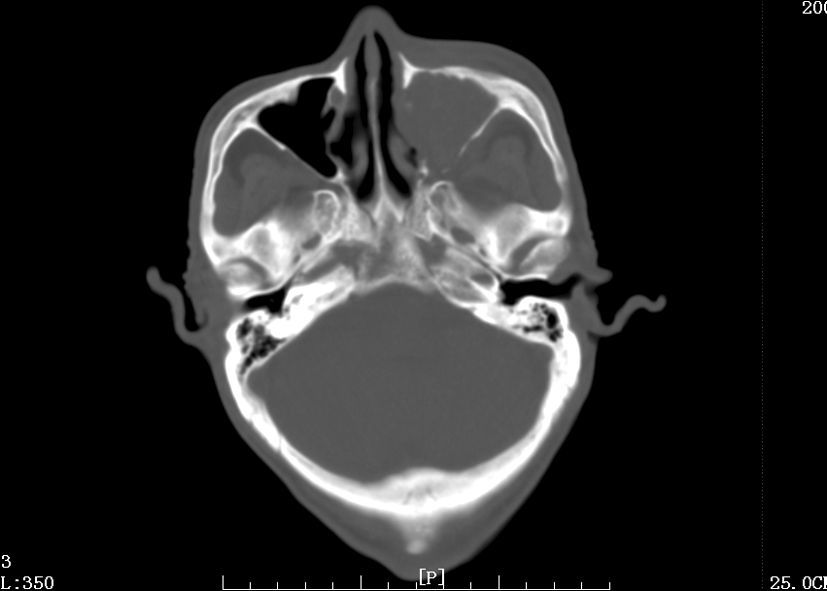
\includegraphics[width=.7\textwidth,height=\textheight,keepaspectratio]{./images/Image00133.jpg}
 \captionsetup{justification=centering}
 \caption{左上颌窦NHL\\{\small 左侧上颌窦腔内软组织肿块,骨质破坏相对较轻}}
 \label{fig5-11}
  \end{figure} 

\textbf{【鉴别诊断】}

1.鼻息肉:好发于中鼻道,软组织密度不均,骨质可有吸收或增生改变,鼻前庭和局部皮肤多无累及。

2.血管纤维瘤:多起于后鼻腔,向前后浸润,病变范围广泛,有明显强化。

3.内翻乳头瘤:常呈一侧中、下鼻甲处不规则软组织肿块,邻近结构为推压移位。双侧肿块多位于鼻腔后部,肿瘤可经后鼻孔侵及对侧。

4.上颌窦癌:窦壁骨质破坏及其周围软组织肿块较明显,鼻腔受累较晚,且易发生中心坏死。而NHL多位于居中线区,骨质破坏不显著,其相应部位软组织块影常大于骨质破坏范围是重要的鉴别点。

5.鼻咽癌:NHL的以下特征有助于与鼻咽癌鉴别:①咽缝存在;②愈往深层病变越轻;③颅底骨质无破坏;④病灶多中心、多部位。

\protect\hypertarget{text00013.html}{}{}

